\documentclass[a4paper,11pt]{book}
\usepackage[utf8]{inputenc}
\usepackage[center,font=footnotesize,labelfont=bf]{caption}
\usepackage{graphicx}
\usepackage[hidelinks]{hyperref}
\usepackage[english, spanish]{babel}
\usepackage{url}
\usepackage{amsfonts}
\usepackage{listings}
\usepackage{float}
\usepackage{afterpage}
\usepackage[babel]{csquotes}
\usepackage[backend=biber,style=apa]{biblatex}
\DeclareLanguageMapping{spanish}{spanish-apa}
\addbibresource{main.bib}
%\bibliography{main}

\DefineBibliographyExtras{spanish}{%
	\let\finalandcomma\empty
	\let\finalandsemicolon\empty
}
\setlength\bibitemsep{1.5\itemsep}
\usepackage{chngcntr}
\counterwithout{section}{chapter}
\usepackage[toc,page]{appendix}

\addto\captionsspanish{%
	\renewcommand\appendixtocname{Anexos}
	\renewcommand\appendixname{Anexo}
	\renewcommand\appendixpagename{Anexos}
}

\usepackage{fancyhdr}
\pagestyle{fancy}
\fancyhf{}
\fancyhead[LO]{\rightmark}
\fancyhead[RE]{\rightmark}
\fancyhead[RO,LE]{\textbf{\thepage}}

\renewcommand{\sectionmark}[1]{\markright{\textbf{\thesection. #1}}}

\usepackage{colortbl,longtable}
\definecolor{gray97}{gray}{.97}
\definecolor{gray75}{gray}{.75}
\definecolor{gray45}{gray}{.45}
\definecolor{gray30}{gray}{.94}


\lstset{ frame=Ltb,
	framerule=0.5pt,
	aboveskip=0.5cm,
	framextopmargin=3pt,
	framexbottommargin=3pt,
	framexleftmargin=0.1cm,
	framesep=0pt,
	rulesep=.4pt,
	backgroundcolor=\color{gray97},
	rulesepcolor=\color{black},
	%
	stringstyle=\ttfamily,
	showstringspaces = false,
	basicstyle=\scriptsize\ttfamily,
	commentstyle=\color{gray45},
	keywordstyle=\bfseries,
	%
	numbers=left,
	numbersep=6pt,
	numberstyle=\tiny,
	numberfirstline = false,
	breaklines=true,
}

\usepackage[titles]{tocloft}
\renewcommand{\cftsecleader}{\bfseries\cftdotfill{\cftsecdotsep}}
\renewcommand{\cftsecfont}{\normalfont\bfseries}


%   Generate the environment for the abstract:
\newcommand\summaryname{Abstract}
\newenvironment{abstract}%
{\small\begin{center}%
		\bfseries{\summaryname} \end{center}}


%   Generate the environment for the abstract:
\newenvironment{resumen}%
{\small\begin{center}%
		\bfseries{Resumen} \end{center}}



% ADD BLANKPAGE
\newcommand\blankpage{
    \null
    \thispagestyle{empty}
    \addtocounter{page}{-1}
    \newpage
}
%%%%%%%%%%%%%%%%%%%%

% ADD A NEW DEPTH SECTION (PARAGRAPH)
\usepackage{titlesec}
\usepackage{amsmath}
\setcounter{secnumdepth}{4}
%\titleformat{\paragraph}{\normalfont\normalsize\bfseries}{\theparagraph}{1em}{}
%\titlespacing*{\paragraph}{0pt}{3.25ex plus 1ex minus .2ex}{1.5ex plus .2ex}
\titleformat{\section}[block]{\Large\bfseries}%
{\thesection}
{5mm}
{}
\titleformat{\subsection}[block]{\large\bfseries}%
{\thesubsection}
{5mm}
{}
\titleformat{\subsubsection}[block]{\bfseries}%
{\thesubsubsection}
{5mm}
{}
\titleformat{\paragraph}[block]{\bfseries}%
{\theparagraph}
{5mm}
{}

% END OF ADDING
\setcounter{tocdepth}{4}
\setcounter{secnumdepth}{4}

\raggedbottom
\begin{document}
\nocite{*}

	\begin{titlepage}
		\afterpage{\blankpage}
		\centering
		
\includegraphics[width=0.8\textwidth]{imagenes/logo_ugr.jpg}\par\vspace{1cm}
		{\scshape\LARGE Universidad de Granada \par}
		\vspace{1cm}
		{\scshape\Large Proyecto fin de Doble Grado en Ingenier\'ia Inform\'atica y Matem\'aticas\par}
		\vspace{1.5cm}
		{\huge\bfseries Una estrategia para bolsa basada en algoritmos evolutivos y su implementaci\'on en una plataforma de trading\par}
		\vspace{0.2cm}
		\noindent\rule{\textwidth}{1pt}
		\vspace{2cm}

		\vfill
		Autor\par
		{\large Miguel \'Angel Torres L\'opez}
		\vfill
		Director\par
		{\large Jose Manuel Zurita L\'opez}
		
		\vfill
		
		% Bottom of the page
		{\large Granada, \today\par}
			
	\end{titlepage}
		

\vskip 4cm

\textbf{Agradecimientos}\\

En este proyecto se intenta predecir el mutable\\
valor de las acciones de bolsa.\\
A pesar de esto, doy mi agradecimiento\\
a la única acci\'on que no necesita ninguna predicci\'on:\\
el apoyo de los que siempre est\'an ah\'i,\\
bien por afecto, bien por profesionalidad.

\newpage

\begin{abstract}
	El mercado de valores ha sido durante muchos años el lugar donde se invierte más dinero. Poseer informaci\'on privilegiada sobre los activos burs\'atiles es cada vez m\'as importante, pues dan a empresas e inversores la capacidad de tomar mejores decisiones econ\'omicas. Con el objetivo de conseguir estos conocimientos, se ha dise\~nado e implementado un algoritmo evolutivo basado en \'arboles de decisi\'on. Estos \'arboles, construidos a partir de la herramienta gen\'etica, se componen de indicadores burs\'atiles cl\'asicos que conforman las reglas del modelo de inversi\'on.\\
	
	Esta t\'ecnica, a pesar de tener un componente aleatorio, puede reporta unos resultados exitosos, especialmente en el caso de las inversiones a largo plazo. No obstante, en inversiones a corto plazo o tendencias demasiado inestables los beneficios son m\'as modestos e, incluso, se producen p\'erdidas.
	
	A partir de este proyecto, se propone el uso de m\'ultiples herramientos y modelos de la bolsa de valores para adquirir una mejora de los conocimientos del mercado que, si bien est\'a repercutido por factores ajenos a los indicadores, puede ser perfilado mediante estos.
	
	\vspace{2cm}
    \noindent\textbf{Palabras clave:} predicci\'on de bolsa, miner\'ia de datos, algoritmo evolutivo, \'arbol de decisi\'on, indicadores burs\'atiles
\end{abstract}

\newpage
\selectlanguage{english}
\begin{abstract}
    The stock market has been for many years the place where most money is invested on. To own insider information about the stock asset is becoming increasingly important cause of the better decisions that investors and business are able to take. In order to achive that knowledge, an evolutionary algorithm based on decision trees has been designed and developed.
    
    We find researches where the focus is to know the exact price that the asset will reach in some time. Other ones try to classificate the trend where the stock is involved or even the one where it will be. At this end-of-grade project, we work with a different point of view. We are not interested anymore on the stock value. Instead of that, a buy and sell signal model is going to be built. That means that the knowledge we aqcuire is not the stock value but the time where we should buy or sell.\\
    
    To obtain the decision tree who will send us the signal we need some trading tools. 
    
    As Python is the language selected, \textit{backtrader}, a backtesting framework, is going to be used. This framework let us to dislinkage the backtesting process from the main evolutionary algorithm developed. Besides, \textit{backtrader} gives us some plotting amenities, to get a better analysis, and a strong parallel processing, that will be necessary due to time limitations. 
    
    After that, we need to get the stock market data we are going to work with. We check multiple ways to take them to \textit{backtrader} but, the best solution seems to be \textit{pandas\_datareader}.
    
    Finally, as we need to calculate numerous times the indicator values at different days, we work with an analysis package for that porpouse, \textit{TA-Lib}. The package allows to work out many classic indicators from a period at once, instead of calculate them day per day.\\
    
    Once we have introduced the tools, we are prepared to build the algorithm. Because the aim is to develop a tree decision model we must first explain the tags or classes. 
    
    The model must send two different signals: buy and sell. However, a three tag tree is proposed due to some undeterminated moments at the stock market. So, the three tags are: Buy, if we should send a buy signal, sell, if we should send a sell signal, and stop, if the model can not take any previous tag.
    
    Next, we need to design how conditions on tree nodes are built. The tree is formed with rules that look like 
    \[indicator(params) <= pivot\]
    
    \begin{itemize}
	    \item \textit{Indicator} is an indicator taken from the list (MACD, ATR, ROC, EMA, SMA, Momentum, HILL, RSI, OBV, AD, TRANGE, Bollinger Band High, Bollinger Band low).
	    \item \textit{Params} is a variable list of parameters that depends on the indicator.
	    \item \textit{Pivot} is a real number that splits the day on two branches, the positive condition one and the negative one.
    \end{itemize}
    
    As expected, we just manage binary trees.\\
    
    At this point, we define the evolutionary algorithm. Our first approach was building the first population with random procedures. Further experiment with heuristic methods gave better results for the first generation. Despite of the time wasted on it, we choose to warm up the population by building them with randomness for indicators but entropy functions for pivots.\\
    
    After that, each tree is evaluated with the fitness function, that is, the simulation of a training period where \textit{backtrader} works out the return from invest with each tree based strategy.
    
    The money returned by each tree is used to set the crossover probability, that is, the probability of being selected to generate a new tree. That probability is proportional to the score achieved on the simulation.\\
    
    In order to get the new population, the crossover is managed as next:
    
    First select a random node from each tree. Note that selected nodes could be roots, the top nodes, but could not be a leaf as this will produce a nonsense decision tree.
    
    Then, the subtrees under the choosen nodes are swapped. That way, we have two new trees with some different conditions.
    
    Note that params and pivots in the condition are not changed with that crossover. So thats the point to introduce the mutation. After each new tree generation, the mutation factor is mandatory. Four mutation methods are devoloped. 
    \begin{itemize}
    	\item Indicator mutation. Selects a new indicator from the above list. That triggers to change parameters and pivot.
    	\item Pivot mutation. Following a normal distribution, introduce a random noise on pivot.
    	\item Parameters mutation. Change the parameters by taking a new one based on a discrete uniform distribution, if the parameter is discrete, or on a normal distribution, if the parameter is continuous.
    	\item Leaf mutation. That is a special mutation that change the tag of a leaf. As we cant take leaves for crossover, those will remain down the same indicator at every population. This relation was set up in the first generation, so it should not be correct.  
    \end{itemize}
    
    Once the new population is finally generated, the process starts again by evaluating the trees. \\
    
    Due to time limit, some improvements are made to reduce the execution time. The first one is the  \textit{backtrader} parallel execution. After that, a deep analysis revealed that most of the time was wasted on taking data from \textit{pandas dataframe}. So, to reduce that a cache to save data closer was developed.\\
    
    Once the algorithm is ready for executions, a window of parameters is proposed to check the best ones. \\
    
    The algorithm seems to learn, reasonably well, the pattern to invest with benefits in the trainning period. Furthermore, buy signals are sent close-fitting to minimums.
    
    However, while investing on test periods, results are not that good. At small periods, minimums are well found, but the model sends sell signals even when commissions are bigger than benefits. 
    
    At long investing periods, signals are not sent frecuently. That produce \textit{Buy\&Hold} strategies at uptrends and no buys at downtrends.
    
    Despite of the results, the algorithm builds models that learn well the patterns on the training period. To improve results we suggest to use the evolutionary algorithm with a complementary algorithm that could help the first by testing the trend.
    
    Through this project, stock indicator rules are prove to be given useful knowledge to understand the market situation. Nevertheless, a prediction algorithm with them seems not worth at unsettled trend markets.  
    
      
    
    \vspace{2cm}
    \noindent\textbf{Keywords:} stock prediction, data mining, evolutionary algorithm, decision tree, stock indicator
\end{abstract}
\selectlanguage{spanish}
\newpage

\tableofcontents
\newpage
\listoffigures

\newpage

\section{(Introducci\'on) Predicci\'on en el mercado de valores}

Una de las formas más sencillas, y a la vez dif\'iciles, de enriquecerse es la compra de bienes y posterior venta a un precio mayor. La ganacia se produce si se consigue que la diferencia entre el precio de compra y el precio de venta sea mayor que los costes producidos a raz\'on de esa transacci\'on. En el mundo de los negocios la compra y la venta de bienes aparecen en casi todos los sectores econ\'omicos. Por ejemplo:\\

\begin{itemize}
    \item Distribuci\'on de mercancias. Hay empresas que se dedican a comprar mercancias en un punto y distribuirlas por otras zonas a un precio mayor. El coste de este ejercicio reside en el transporte. La empresa debe asegurar que los costes de transportes no superan a la diferencia de precio entre compra y venta.
    
    \item Especulaci\'on de terrenos o edificios. Un poco m\'as cara que la anterior, la compra, y posterior venta, de edificios puede producir beneficios. Las empresas que se dedican a esto tienen en cuenta las posibles construcciones que se van a hacer por la zona que, posiblemente, elevar\'an el valor del inmueble y har\'an el negocio posible. Mantener terreno conlleva un pago de impuestos, que tendr\'a que ser cubierto con el beneficio de la venta. Pero, en este caso, los inmuebles se pueden alquilar para sacar un beneficio continuo.
\end{itemize}

Del mismo modo, el mercado de valores brinda una posibilidad para extraer beneficio con la compra y venta. Se compran acciones a un precio determinado y se intentan vender a otro m\'as alto. Si se tiene informaci\'on adicional que nos d\'e certeza sobre la subida del precio de la acci\'on entonces el negocio es seguro. Si, por el contrario, no se dispone de informaci\'on, el valor de las acciones podr\'ia bajar y provocar una p\'erdida de dinero.\\

Por tanto, tener conocimiento sobre el estado del mercado sit\'ua a empresas y particulares en posiciones ventajosas. Es por esto que, siguiendo distintas estrategias, las personas que invierten en bolsa intentan extraer informaci\'on sobre la situaci\'on actual y futura del mercado.\\

A lo largo de este proyecto se va a intentar extraer informaci\'on a partir del hist\'orico de valores del mercado, es decir, vamos a utilizar el estado del mercado en un per\'iodo pasado para predecir el estado futuro. \\


\subsection{Precedentes en la predicci\'on de bolsa}
El primer mercado de valores se sit\'ua en el siglo XVII. Seg\'un afirma Beattie (2017) en la revista digital Investopedia, la primera empresa en ofrecer acciones se situar\'ia en B\'elgica, promovida por la incipiente econom\'ia generada en las colonias de Asia. \\

A lo largo de tantos a\~nos de vida, los valores burs\'atiles se han intentado predecir de muchas formas. A medida que la sociedad avanza y se van creando nuevas herramientas, los modelos de predicci\'on van evolucionando y se hacen m\'as complejos.\\

En la actualidad podemos distinguir varias agrupaciones de an\'alisis de bolsa:\\

\begin{itemize}
    \item \textbf{An\'alisis chartista}. Debe su nombre a la palabra inglesa \textit{chart}. Las estrategias de esta agrupaci\'on se valen de reglas gr\'aficas aplicadas sobre \'indices o sobre el propio valor de la acci\'on. Esas reglas gr\'aficas advierten de series temporales, como las ondas de Elliot (Elliot, 1994), o de tendencias y rupturas (Gartley, 1935). \\
    
    Esta estrategia se lleva utilizando mucho tiempo por su simplicidad y su f\'acil comprensi\'on y evaluaci\'on.
    Su \'exito se debe probablemente a este hecho, y es que con una sencilla herramienta gr\'afica se pueden deducir, a gran escala, algunas subidas o bajadas de los valroes de bolsa.
    
    \item \textbf{An\'alisis de \'indices o indicadores}. Esta modalidad de an\'alisis se basa en el uso de estad\'isticos. En el campo de la estad\'istica, los estad\'isticos son valores que representan una determinada caracter\'istica de la variable a la que refiere. En el caso de los indicadores, informan del estado de uno o varios valores distintos de la bolsa. Una de las publicaciones con m\'as renombre es la teor\'ia de Dow\footnote{Hamilton, W. P. (1922). \textit{The Stock Market Barometer; a Study of Its Forecast Value Based on Charles H. Dow's Theory of the Price Movement}, Harper \& Bros., Nueva York}, cuyo autor, Charles H. Dow, fue el fundador del \textit{Wall Street Journal}, diario en el que publicaba sus principios para invertir en bolsa. \\
    
    Seg\'un la variable que resume el indicador podemos hablar de varios tipos. El primer tipo son los indicadores que representan la situaci\'on general de la bolsa de un pa\'is, por ejemplo el IBEX35 (35 empresas con m\'as capital de Espa\~na). Otro grupo de indicadores son los representan la situaci\'on de las empresas que se dedican a un sector particular, como el  SX7E (bancos de los paises europeos).
    Por \'ultimo hay \'indicadores que aportan informaci\'on estad\'istica sobre un solo valor, por ejemplo la EMA (Media M\'ovil Exponencial).
\end{itemize}

Este proyecto se centra en el an\'alisis de indicadores de un solo valor. En concreto, como se ver\'a a lo largo del trabajo, se propone un modelo basado en \'arboles de decisi\'on construidos a partir de un algoritmo gen\'etico. Los \'arboles de decisi\'on son, a grandes rasgos, estructuras que permiten crear una jerarqu\'ia de condiciones que tienen como conclusi\'on de las mismas una clasificaci\'on. En el caso que nos compete, la clasificaci\'on corresponder\'a a decidir si es un buen momento para comprar, para vender o para ninguno de los dos. En el apartado \ref{sec:algorithm} se entrar\'a con m\'as profundidad en este modelo. \\



\subsection{Tipos de informaci\'on extra\'ible a partir de \'arboles}
Podemos encontrar en la bibliograf\'ia varios modelos basados en \'arboles que, seg\'un la informaci\'on que persiguen conseguir, se pueden dividir en varios grupos. En este punto debemos hacer notar que existen otras formas y herramientas de extracci\'on informaci\'on o predecci\'on, pero por la naturaleza de nuestra propuesta nos centraremos en las estrategias basadas en \'arboles. Debido al caracter motivacional de la secci\'on, no se entra en profundidad en estos conceptos. No obstante, la definici\'on de \'arbol puede verse posteriormente en el apartado \ref{sec:Decision_tree}.

    \subsubsection{Informaci\'on total}
    
    El m\'as ambicioso de los objetivos de un an\'alisis de bolsa es el de encontrar una forma de predecir el valor exacto de un valor burs\'atil en un instante de tiempo futuro. Encontramos entonces una funci\'on $f:\Omega \rightarrow \mathbb{R}$ donde $\Omega$ es un conjunto de indicadores del valor a predecir en un instante pasado o presente y la imagen, contenida en $\mathbb{R}$ es el valor predicho para un instante en el futuro.\\
    
    El instante predicho cambia seg\'un el autor del estudio (pueden ser horas, d\'ias o semanas), normalmente, cuanto m\'as alejado est\'a del instante en el que se eval\'ua $f$ del instante que se pretende predecir, mayor es el error.\\
    
    La funci\'on $f$ se puede representar como un \'arbol en el que en los nodos se sit\'uan operaciones (usualmente unarias o binarias) y las hojas contienen par\'ametros de la funci\'on $f$ o valores constantes. La funci\'on se eval\'ua desde las hojas hasta el nodo ra\'iz. \\
    
	\begin{figure}[H]
		\centering
    	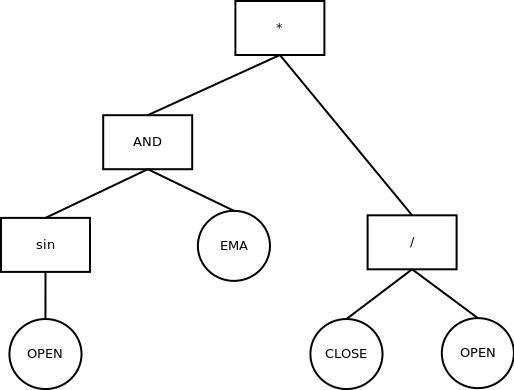
\includegraphics[scale=0.5]{imagenes/arbol_inf_comp.png}
    	\caption[Ejemplo de \'arbol de programaci\'on gen\'etica]{Ejemplo de \'arbol de programaci\'on gen\'etica.\\ Fuente: elaboraci\'on propia.}
    	\label{fig:inf_compl}
    \end{figure}
    
    En la figura \ref{fig:inf_compl} puede verse un \'arbol de este tipo. De este se puede extraer la funci\'on \\
    $f($OPEN, CLOSE, EMA$) = (sin($OPEN$)$ AND EMA$) * ($CLOSE/OPEN$)$\\ que, dados unos valores para la apertura, el cierre y la media m\'ovil exponencial, nos devuelve el valor en el instante futuro.\\
    
    Para ajustar los \'arboles se usa un algoritmo gen\'etico con funci\'on \textit{fitness} el error medio cuadr\'atico entre el valor predicho y el error real (Sheta, 2013). Se comentar\'a con profundidad el funcionamiento de los algoritmos gen\'eticos m\'as adelante. Tambi\'en existe otra variante basada en el \textit{Conditional Sharpe Ratio} aplicada en Esfahanipour (2011) y Mousavi (2014).\\
    
    Por \'ultimo, una funci\'on \textit{fitness} algo diferente es puntuar cada estrategia a partir del beneficio simulado obtenido en un periodo de tiempo (Potvin, 2004).\\
    
     Si se consiguiese hallar una funci\'on $f$ con un error nulo, obtendriamos una informaci\'on perfecta con la que podr\'iamos conseguir el m\'aximo beneficio en bolsa. No obstante, este tipo de modelos es demasiado ambicioso. Computacionalmente es pesado y la funci\'on resultante no es, en casi todos los casos, interpretable.\\
     
     
     \subsubsection{Informaci\'on de tendencias}
     
     En lugar de buscar una predicci\'on exacta del valor en el futuro, podemos estar interesados en obtener informaci\'on sobre la tendencia de un valor, es decir, si est\'a en un periodo ascendente o descendente. \\
     
     Este m\'etodo puede ser visto como una relajaci\'on del m\'etodo desarrollado en el apartado anterior. Aunque el paso de una imagen continua ($\mathbb{R}$) a una imagen discreta (sube, baja, se queda igual) nos obliga a realizar otro tipo de \'arboles. En este caso se suele proponer un \'arbol de decisi\'on con tres etiquetas. Pero no vamos a entrar en detalle aqu\'i en esta herramienta, ya que ser\'a explicada en profundidad en el apartado \ref{sec:Decision_tree}.\\
     
     Estos modelos de informaci\'on son bastante m\'as sencillos de interpretar. Pero, por contra, son bastante m\'as imprecisos. El modelo nos dice la tendencia que tendr\'a el valor. Sin embargo, seg\'un los objetivos de inversi\'on, las comisiones u otras situaciones econ\'omicas, esta informaci\'on podr\'ia no ser suficiente para sacar beneficios.\\
     
     Para profundizar en la extracci\'on de este tipo de informaci\'on se sugiere ver Nair (2010) o Huang (2008).\\
     
     
     \subsubsection{Informaci\'on de se\~nales de compra y venta}
     
     A medio camino entre los dos tipos de informaci\'on anteriores tenemos los modelos de señales, mediante los cuales, los m\'as importante no es conocer el valor de la acci\'on, si sube o si baja, sino buscar un modelo que nos diga cuando comprar y cuando vender. A estas advertencias de los modelos de compra y venta se le llaman se\~nales de compra y venta. Cabe decir que se puede hacer una extensi\'on del modelo para que no tenga una decisi\'on binaria, por ejemplo un modelo de cuatro etiquetas: compra discreta, venta discreta, compra masiva y venta masiva. \\
     
     De este tipo de extracci\'on de informaci\'on hay menos ejemplos, que suelen estar ejecutados a partir de varios \'arboles de salida booleana, cada uno de ellos asociado a una se\~nal. En Myszkowski (2010) podemos ver un claro ejemplo con dos \'arboles, uno que indica la compra y otro que indica la venta.\\
     
     	\begin{figure}[H]
			\centering\leftskip=-10px
			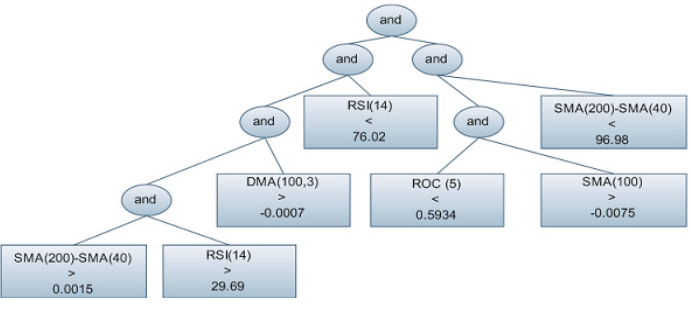
\includegraphics[scale=0.8]{imagenes/tree_halfinfo.png}
			\caption[Ejemplo de \'arbol de señales de compra]{Ejemplo de \'arbol de señales de compra. \\Fuente: Myszkowski (2010)}
			\label{fig:tree_half_info}
		\end{figure}
		
	En la figura \ref{fig:tree_half_info} se muestra un \'arbol de se\~nal de compra. N\'otese que en los nodos hoja siempre hay una condici\'on booleana que puede contener un solo indicador o, en caso especial, dos.\\
	
	\subsection{Objetivo del proyecto}
	La importancia de obtener informaci\'on exclusiva sobre el estado de la bolsa es evidente, ya que esto te permite invertir en bolsa con mayor posibilidad de sacar beneficios que si se realizara por mera intuici\'on.\\
	
	De este modo, siguiendo el desarrollo realizado en los antecedentes aportados, se propone conseguir los siguientes objetivos principales:
	
	\begin{itemize}
	    \item Dise\~nar, y desarrollar posteriormente, un algoritmo gen\'etico basado en \'arboles que permita extraer informaci\'on de se\~nales de compra y venta.
	    \item Debido al coste computacional de los algoritmos gen\'eticos, se busca implementar dicho algoritmo de la forma m\'as eficiente posible, en especial la funci\'on de evaluaci\'on.
	    \item Ejecutar en distintas tendencias burs\'atiles y comparar los resultados con los aportados en la bibliograf\'ia.
	\end{itemize}
	
	A pesar de que el hist\'orico de datos es clave para predecir los valores futuros, el mercado de valores a menudo se ve influenciado por otros factores no predecibles (noticias, pol\'itica, guerras o cat\'astrofes ambientales, por ejemplo). Por tanto, aunque el modelo predicho sea muy bueno, siempre habr\'a un punto de incertidumbre que nunca estaremos en condiciones de analizar.\\
	
	En consecuencia, partimos de la idea de que la inversi\'on perfecta no se puede conseguir, al menos de forma juiciosa y sistem\'atica. No obstante, a\~nadimos un punto adicional a los objetivos que, a priori, es complicado alcanzar:
	
	\begin{itemize}
	    \item Mejorar los resultados obtenidos en la bibliograf\'ia en los distintos mercados de valores.
	\end{itemize}
	
	
\newpage

	\subsection{Herramientas de simulaci\'on}		
	El prop\'osito central de este proyecto es encontrar un modelo con estrutuctura de \'arbol que sea capaz de invertir en bolsa de forma beneficiosa. Puesto que la ejecuci\'on del modelo es necesaria para medir su bondad, hay que trabajar en un entorno de pruebas en el que poder hacer ensayos. Este entorno no debe ser la bolsa real, porque simular grandes periodos costar\'ia el mismo tiempo que la longitud del periodo y, adem\'as, se estar\'ia haciendo con dinero real, con todas las dificultades que esto puede tener.\\
	
	En su lugar, las plataformas de \textit{backtesting} ofrecen las simulaciones que se necesitan. El \textit{backtesting} es el proceso que permite simular un periodo de bolsa e invertir con una estrategia particular de forma sistem\'atica. A continuaci\'on, se mencionan algunas plataformas y un peque\~no an\'alisis de cada una para discernir cu\'al es mejor para esta tarea.\\ 
	
	
		\subsubsection{MetaTrader5}
		
    	\textit{MetaTrader5} es una software, disponible en versi\'on escritorio y en versi\'on web, con el que se pueden comprar y vender acciones en tiempo real pero de forma simulada, es decir, sin participar con dinero real. Es una plataforma ampliamente usada y, por tanto, es f\'acil encontrar ejemplos iniciales o ayuda t\'ecnica. Por comentar una de las facilidades, en la p\'agina web de la plataforma\footnote{\url{https://www.metatrader5.com} [\'Ultima consulta 10 de Julio de 2019]} se nos ofrece una demo gratuita con acceso a la mayor\'ia de los recursos, aunque hay algunas herramientas de pago.\\
		
		La programaci\'on de las estrategias se organiza en varios archivos con unas especificaciones concretas. Adem\'as, existe una tienda empotrada en la plataforma para comprar y vender estrategias, \'indices o bibliotecas con otros usuarios. Cada producto est\'a puntuado por los usuarios que lo han usado. A priori, esto puede ser bastante \'util para comparar la estrategia propuesta en el proyecto con otras estrategias cl\'asicas o con las estrategias mejor puntuadas en la plataforma.\\
		
		A pesar de todas estas ventajas, no usaramos \textit{MetaTrader5} por ser de car\'acter privativo. Asimismo, el lenguaje de programaci\'on de las estrategias es \textit{MQL5}, un lenguaje propio de la plataforma, que nos impide usar con facilidad bibliotecas externas.\\
	
		\subsubsection{Backtrader}\label{sec:backtrader}
		
		\textit{Backtrader} es un \textit{framework} de libre licencia desarrollado en el lenguaje \textit{Python}. La p\'agina web de la plataforma\footnote{\url{https://www.backtrader.com} [\'Ultima consulta 10 de Julio de 2019]} contiene una amplia documentaci\'on en la que se explican todos los componentes de este \textit{framework}. Tambi\'en se encuentran, en el mismo lugar, el m\'etodo de instalaci\'on y un tutorial de iniciaci\'on para simulaci\'on de bolsa.\\
		
		La herramienta contiene indicadores ya programados, aunque se permite hacer m\'as de forma manual.  Instalando una librer\'ia adicional se pueden generar gr\'aficas de ganancias en un periodo de simulaci\'on. Este desacoplamiento de la parte gr\'afica no supone un gran problema porque en la instalaci\'on viene integrada la opci\'on para instalar todo, tal y como se ver\'a en el siguiente apartado.\\
		
		
		\paragraph{Instalaci\'on}\label{sec:install}
		
		Pasamos pues, a ilustrar la instalaci\'on de \textit{backtrader}. La instalaci\'on puede hacerse en cualquier sistema operativo que soporte \textit{Python} pero, en lo que sigue, se supondr\'a que el sistema es \textit{Ubuntu}. \\
		
		En primer lugar, es preciso tener la versi\'on 2.7 de \textit{Python}, como se indica en la documentaci\'on de \textit{backtrader}\footnote{\url{https://www.backtrader.com/docu/index.html} [\'Ultima consulta 10 de Julio de 2019]} que se ubica en su p\'agina web. Para comprobar la versi\'on, se puede usar el comando \textit{python -Version}. En caso de no tener instalado \textit{Python} o no tener la versi\'on indicada, se puede instalar usando \textit{sudo apt-get install python2.7}.\\
		
		El \textit{framework backtrader} est\'a disponible desde el c\'odigo fuente en \textit{Github}. No obstante, es m\'as c\'omodo usar la versi\'on para el instalador de paquetes de \textit{Python, pip}. Si no se tiene instalado \textit{pip}, la instalaci\'on se realiza con el comando \textit{sudo apt-get install python-pip}.\\
		
		Una vez llegados a este punto, se puede optar por una versi\'on con posibilidad de generar gr\'aficas o una versi\'on m\'as ligera sin esta posibilidad. Para facilitar el an\'alisis de resultados, se recomienda instalar la versi\'on con gr\'aficas. Su instalaci\'on se ejecuta con el comando \textit{pip install backtrader[plotting]}, como podemos ver en la figura \ref{fig:pip_backtrader}. Para instalar una versi\'on m\'as ligera, se usa el mismo comando quitando la directiva \textit{[plotting]}. En este caso se instala una versi\'on similar pero sin la posibilidad de hacer gr\'aficas.\\
		
		\begin{figure}[H]
			\centering
			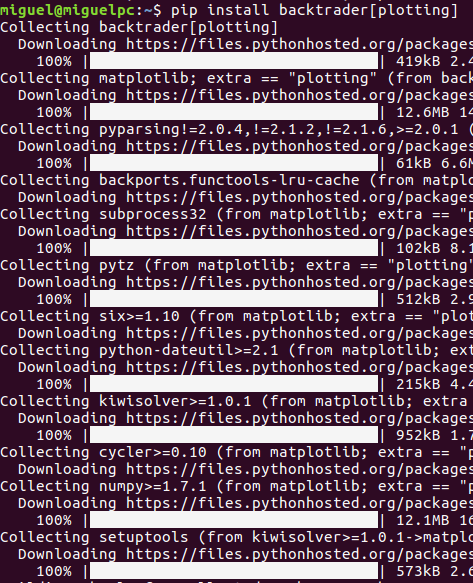
\includegraphics[scale=0.4]{imagenes/pip_backtrader.png}
			\caption[Resultado de instalar backtrader con plotting]{Resultado de instalar backtrader con plotting.\\ Fuente: elaboraci\'on propia.}
			\label{fig:pip_backtrader}
		\end{figure}
		
		La instalaci\'on de backtrader conlleva la instalaci\'on de otros paquetes adicionales con los que tiene dependencias. Entre ellos hay que destacar el paquete \textit{numpy}, que m\'as tarde nos ser\'a \'util como herramienta matem\'atica para generar distribuciones estad\'isticas.\\
		
		
		\paragraph{Preparaci\'on del entorno}
		
		Una de las estructuras de datos m\'as comunes en \textit{backtrader} son las l\'ineas. Una l\'inea no es m\'as que un conjunto de datos ordenados por orden cronol\'ogico, del m\'as antiguo al m\'as moderno. Por ejemplo, al hablar de un valor de mercado tenemos 5 l\'ineas b\'asicas: valor de apertura, valor de salida, valor m\'aximo, valor m\'inimo y volumen de compra/venta. \\
		
		En t\'erminos de inform\'atica, para acceder a los elementos de cada l\'inea, hay que tener en cuenta que no se puede usar la indexaci\'on de un vector como en un lenguaje de programaci\'on com\'un. En su lugar, el \'indice 0 representa el instante actual y, a partir de este, se cuentan con los n\'umeros enteros las posiciones de los dem\'as. Hay que aclarar que para acceder a instantes anteriores usaremos \'indices negativos, como por ejemplo:\\
		
		\begin{lstlisting}[basicstyle=\tiny]
	self.sma = SimpleMovingAverage(...)
	valor_actual            = self.sma[0]
	valor_instante_anterior = self.sma[-1]
		\end{lstlisting}
		
		\vspace{0.8cm}
		
		Por tanto, seg\'un el d\'ia que se est\'e simulando, los datos de otro d\'ia concreto se acceden con un \'indice o con otro. De esta forma, suponiendo que se est\'a simulando el lunes y queremos acceder al dato del mi\'ercoles el \'indice es el 2. Si por el contrario se simula el jueves, para acceder al mi\'ercoles se usa el \'indice -1. N\'otese que, por motivos acad\'emicos, no se deben usar los \'indices mayores que 0, ya que esto supondr\'ia tener informaci\'on sobre el futuro y la predicci\'on de la bolsa ser\'ia un fraude.\\
		
		Antes de ver c\'omo crear una estrategia, es preciso ver como se puede simular una prueba introduciendo unos datos y un presupuesto inicial. Para ello, en un archivo con terminaci\'on \textit{.py}, para poder ejecutar con \textit{Python}, se insertar\'a el siguiente c\'odigo:\\
		
		\begin{lstlisting}[basicstyle=\tiny]
from __future__ import (absolute_import, division, print_function, unicode_literals)
		
import datetime
import os.path
import sys
import backtrader as bt # Importar todas las herramientas de backtrader
		
if __name__ == '__main__':
	cerebro = bt.Cerebro()
		
# Crear un paquete de datos
	data = bt.feeds.YahooFinanceCSVData(
	dataname='YAHOO',  # Ruta absoluta donde se encuentran los datos descargados de YAHOO! Finance
# Fecha inicial de los datos
	fromdate=datetime.datetime(2000, 1, 1),
# Fecha final de los datos
	todate=datetime.datetime(2000, 12, 31),
	reverse=False)
		
# Activar los datos en el cerebro
	cerebro.adddata(data)
# Establecer dinero inicial    
	cerebro.broker.setcash(100000.0)
		
	print('Starting Portfolio Value: %.2f' % cerebro.broker.getvalue())
	cerebro.run()   # EJECUTAR BACKTESTING (AHORA MISMO, SIN NINGUNA ESTRATEGIA)
	print('Final Portfolio Value: %.2f' % cerebro.broker.getvalue())
		\end{lstlisting}
		
		\vspace{0.5cm}
		
		N\'otese que se trata de una archivo \textit{Python} en el que solo hemos tenido que importar el paquete \textit{backtrader}. Por tanto, en el caso de necesitar otros paquetes para realizar nuestra estrategia, solo ser\'a necesario incorporarlos de la forma habitual en este lenguaje de programaci\'on.\\
		
		El c\'odigo es ejecutable y funcional, pero hay un problema, no se le ha especificado a la clase \textit{cerebro} cu\'al va a ser la estrategia a seguir. Por este motivo, si se haciera la simulaci\'on, el presupuesto inicial y final no variar\'ian. \\
		
		Para ejecutar el \textit{backtesting} simplemente se ejecuta el \textit{script} de \textit{Python} con el comando \textit{python rutadelscript.py} en la terminal. Seguramente dar\'a un fallo porque la ruta donde deber\'ia estar el fichero con los datos a simular est\'a vac\'ia. Esto era de esperar pues no hemos descargado ning\'un archivo de datos. El desarrollo de este tema se abordar\'a en la secci\'on \ref{sec:get_data}.\\
		
		
		\paragraph{La primera estrategia}
		
		Antes de programar la primera estrategia de \textit{trading}, vamos a ilustrar con una f\'util c\'omo estructurar una clase para que \textit{backtrader} pueda trabajar con ella como estrategia. La estructura b\'asica es una clase con un m\'etodo \textit{\_\_init\_\_} y otro m\'etodo llamado \textit{next}. \\
		
		El primero puede usarse para instanciar y agrupar los datos que requiera nuestra estrategia. El segundo m\'etodo, por su parte, es llamado en cada instante simulado por \textit{backtrader}, considerando que un instante es cada una de las marcas temporales que hay registradas en nuestros datos. Por aclarar esto un poco, si aportamos al \textit{cerebro} unos datos tomados de forma diaria, los instantes son cada uno de los d\'ias. \\
		
		Cabe destacar que, en cada llamada al segundo m\'etodo, solo son accesibles los datos con marcas temporales menores o iguales al instante correspondiente a la llamada. Existe, no obstante, una forma de saltarse esta regla y conseguir informaci\'on de instantes posteriores. Pero como se especific\'o en el apartado anterior, no es de inter\'es acad\'emico.\\
		
		Veamos un ejemplo b\'asico en el que, en cada instante, se imprime en pantalla el precio actual del valor:\\
		
		\begin{lstlisting}[basicstyle=\tiny]
# Crear una estrategia
class TestStrategy(bt.Strategy):

	def log(self, txt, dt=None):
		dt = dt or self.datas[0].datetime.date(0)
		print('%s, %s' % (dt.isoformat(), txt))
	
	def __init__(self):
	# Guarda una referencia de la linea de valores de cierre
		self.dataclose = self.datas[0].close
	
	def next(self):
	# Muestra por pantalla el valor de cierre
		self.log('Close, %.2f' % self.dataclose[0])
		\end{lstlisting}
		
		Al ejecutar el \textit{cerebro} con esta estrategia, veremos el valor de cierre de cada instante y, si los datos lo facilitan, la marca temporal asociada a cada instante.\\
		
		Para activar la estrategia es necesario indicar al \textit{cerebro} la clase creada con la siguiente l\'inea, que puede ser situada justo despu\'es de indicar el presupuesto inicial:\\

		\begin{lstlisting}[basicstyle=\tiny]
    # Registrar estrategia
    cerebro.addstrategy(TestStrategy)
		\end{lstlisting}	
		
		\vspace{0.4cm}
		
		De este modo, la estrategia est\'a completa, pero en ning\'un instante se realizan compras o ventas. Para nuestro posterior estudio es imprescindible introducir estas acciones. Sin embargo, por motivos de espacio y tiempo, no entraremos en profundidad en todos los aspectos de la compraventa.\\
		
		Veamos el c\'odigo de la primera t\'actica de inversi\'on que nos muestra el funcionamiento de las \'ordenes burs\'atiles:\\
		
		
		\begin{lstlisting}[basicstyle=\tiny]
class DoubleDownStrategy(bt.Strategy):

	def log(self, txt, dt=None):
		dt = dt or self.datas[0].datetime.date(0)
		print('%s, %s' % (dt.isoformat(), txt))

	def __init__(self):
		self.dataclose = self.datas[0].close

		# Para mantener las ordenes no ejecutadas
		self.order = None

	def notify_order(self, order):
		if order.status in [order.Submitted, order.Accepted]:
			return

		if order.status in [order.Completed]:
			if order.isbuy():
				self.log('BUY EXECUTED, %.2f' % order.executed.price)
			elif order.issell():
				self.log('SELL EXECUTED, %.2f' % order.executed.price)

			self.bar_executed = len(self)

		elif order.status in [order.Canceled, order.Margin, order.Rejected]:
			self.log('Order Canceled/Margin/Rejected')

		self.order = None

	def next(self):
		self.log('Close, %.2f' % self.dataclose[0])
		# Si hay una compraventa pendiente no puedo hacer otra
		if self.order:
			return

		# Si no tengo nada adquirido
		if not self.position:
			if self.dataclose[0] < self.dataclose[-1]:
				if self.dataclose[-1] < self.dataclose[-2]:
					self.log('BUY CREATE, %.2f' % self.dataclose[0])
					self.order = self.buy()

		else:
			# Ya hemos adquirido algo
			if len(self) >= (self.bar_executed + 5):
				self.log('SELL CREATE, %.2f' % self.dataclose[0])
				self.order = self.sell()
		\end{lstlisting}
		
		Aqu\'i se introducen varios conceptos nuevos del \textit{framework}. En primer lugar, las acciones \textit{self.buy()} y \textit{self.sell()}, ejecutadas dentro del m\'etodo \textit{next}, indican que queremos lanzar una orden de compra o de venta, respectivamente. Cuando no se especifica ning\'un par\'ametro, \textit{backtrader} compra o vende al precio de cierre del instante actual una sola acci\'on. Esto no quiere decir que la orden se ejecute en ese instante, sino que, a partir de ese momento y si el precio del producto lo permite, se realizar\'a lo antes posible. N\'otese que una vez lanzada una orden hay que esperar a que se complete o se cancele antes de lanzar otra.\\
		
		Seg\'un lo anterior, esta situaci\'on hace necesario incluir el m\'etodo \textit{notify\_order}. Como su propio nombre sugiere, es llamado cuando una orden cambia de estado o, en otras palabras, es el momento a partir del cual se puede lanzar una nueva orden. En este ejemplo, cuando una orden es completada, mostramos por pantalla si es de compra o venta y el precio de la misma. En ciertas ocasiones, las \'ordenes pueden terminar sin compra o venta. En ese caso, puede haber ocurrido una de dos: ser canceladas, si la estrategia cancel\'o la orden con el comando \textit{self.cancel()}, o rechazas, si bien el dinero disponible era insuficiente para ejecutar la orden.\\
		
		Por \'ultimo, comentaremos la parte l\'ogica de la estrategia presentada en el c\'odigo anterior. En cada instante, el m\'etodo \textit{next} eval\'ua alguno de los siguientes casos:\\
		
		\begin{itemize}
			\item \textbf{Existe una orden lanzada y no terminada.} En este caso debemos esperar. T\'engase en cuenta que \textit{backtrader} permite cancelar una orden, aunque no entraremos en este punto con profundidad.
			\item \textbf{No hay una orden lanzada y tampoco tengo nada comprado.} La cantidad de acciones que se poseen puede comprobarse con \textit{self.position}, que se interpreta como un booleano negativo si no se tiene nada en posesi\'on. En esta situaci\'on solo cabe esperar una orden de compra y, para nuestro ejemplo, la lanzaremos si los \'ultimos dos instantes han bajado su precio de cierre de forma consecutiva.
			\item \textbf{No hay una orden lanzada pero tengo algo comprado.} En este caso, se supone que solo se puede vender, aunque si se tuviese dinero no hay ning\'un problema en comprar m\'as acciones.
			
			 Para ilustrar una nueva herramienta, se propone lanzar una orden de venta cinco instantes despu\'es de haber comprado. Para ello podemos comprobar la longitud de \textit{self} con la funci\'on \textit{len} de \textit{Python}. Esta acci\'on, que puede resultar un tanto extra\~na, es una forma propia del lenguaje \textit{Python} de comprobar las dimensiones de un objeto, en este caso de la compra.
		\end{itemize}
		
		
		\subsubsection{Otras plataformas}

		\begin{itemize}
			\item \textbf{Tradestation.} Permite programar estrategias, pero no hacer \textit{backtesting}. Adem\'as no es de acceso gratuito y obliga a invertir con dinero real.
			
			\item \textbf{Cloud9trader.} Tiene una demo que permite programar estrategias y hacer \textit{backtesting}. Est\'a bien para probar estrategias sencillas basadas en indicadores ampliamente conocidos. No obstante, la programaci\'on hay que hacerla en la ventana del navegador, con un lenguaje propio y sin posibilidad de usar paquetes externos.
			
			\item \textbf{Plus500.} Es una plataforma de \textit{trading} con escasas posibilidades de automatizaci\'on. Tan solo permite algunas  sencillas \'ordenes condicionales preprogramadas.
			
			\item \textbf{PyAlgoTrade.} Es un proyecto desarrollado en \textit{Python} disponible en \textit{Github}. Tiene posibilidad de \textit{backtesting}, de utilizar paquetes externos y, en el caso de estar haciendo \textit{trading} con Bitcoins, de comprar y vender estos de forma real. Los datos del mercado hay que conseguirlos de forma externa en formato CSV.
		\end{itemize}
		
	
	\subsection{Conseguir datos hist\'oricos para realizar \textit{backtesting}}\label{sec:get_data}
		
		Como vamos a usar \textit{backtrader}, una herramienta de simulaci\'on de bolsa en local, vamos a necesitar extraer el hist\'orico de la bolsa. En esta secci\'on veremos c\'omo conseguir los valores hist\'oricos en bolsa de diferentes empresas de forma autom\'atica. A parte de conseguir los datos, veremos la forma de incorporarlos a backtrader para su posterior uso.\\
		
		\subsubsection{Quandl}
		
		\textit{Quandl} es una empresa que re\'une miles de paquetes de datos financieros de todo el mundo. Para acceder a esta informaci\'on es necesario registrarse en su p\'agina web. Una vez tengamos acceso, es posible descargar muchos de los archivos en formato CSV. Aunque quiz\'as la opci\'on m\'as c\'omoda para este proyecto sea utilizar la \textit{API} que ofrece. De esta forma se realiza el acceso a los datos desde \textit{Python}, sin necesidad de hacer una descarga previa a la ejecuci\'on del \textit{script}.\\
		
		Para usar la \textit{API} seguiremos los pasos de instalaci\'on que se pueden encontrar en la documentaci\'on\footnote{\url{https://docs.quandl.com/docs/python-installation} [\'Ultima consulta 10 de Julio de 2019]} de \textit{Quandl}. As\'i, instalamos el paquete \textit{quandl} con el gestor de paquetes \textit{pip}. No obstante, para usar el paquete, debemos indicar la \textit{api\_key} que nos dan al inscribirnos en su p\'agina, \'unica para cada usuario.\\
		
		\begin{lstlisting}[basicstyle=\tiny]
# Crear un paquete de datos con QUANDL
	data = bt.feeds.Quandl(
		dataset='WFE',
		fromdate = datetime.datetime(2016,1,1),
		todate = datetime.datetime(2017,1,1),
		dataname='INDEXES_BMESPANISHEXCHANGESMADRID',
		buffered=True,
		apikey='')
		\end{lstlisting}

			
			

		No obstante, como puede verse en la figura \ref{fig:quandl_install}, \textit{backtrader} tiene alg\'un error interno al usar esta \textit{API}. Error que, como en un foro de la comunidad se apunta\footnote{\url{https://community.backtrader.com/topic/797/quandl-data-feed-futures-data} [\'Ultima consulta 10 de Julio de 2019]}, se debe a una mala lectura de los vectores de datos recibidos. Ante la imposibilidad de resolver este problema, y sin informaci\'on sobre si backtrader lo arreglar\'a, se descarta usar esta forma de adquisici\'on de datos.\\
		
			\begin{figure}[H]
				\centering
				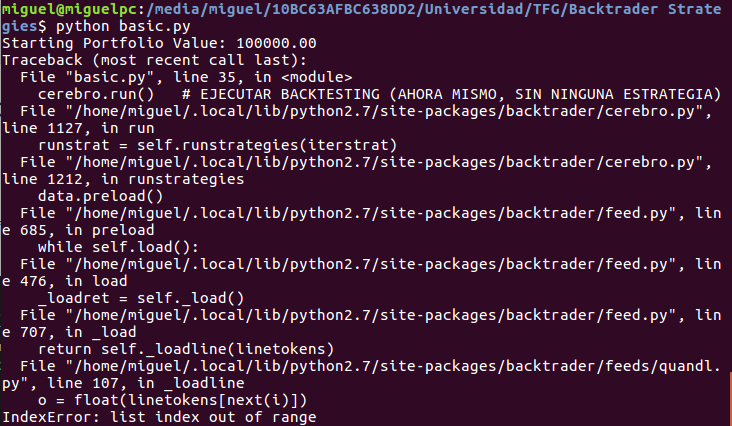
\includegraphics[scale=1.2]{imagenes/quandl_install.png}
				\caption[Ejecuci\'on del script recolectando datos de Quandl]{Ejecuci\'on del script recolectando datos de Quandl. \\Fuente: elaboraci\'on propia.}
				\label{fig:quandl_install}
			\end{figure}
			
			
		\subsubsection{YAHOO! Finance}
				
		Una de las opciones m\'as completas para conseguir los datos es la p\'agina web de \textit{YAHOO! Finance} \footnote{\url{https://finance.yahoo.com}}. Basta con buscar el \'indice o la empresa sobre la que se desean obtener los datos, indicar las fechas y la frecuencia de muestreo y pinchar en el bot\'on de descarga. A continuaci\'on, los datos se descargar\'an en formato CSV con las columnas de fecha, apertura, clausura, m\'aximo, m\'inimo y volumen. Este formato es ampliamente utilizado por la comunidad cient\'ifica para almacenar grandes cantidades de datos.\\
				
		\begin{figure}[H]
			\centering\leftskip=-30px
			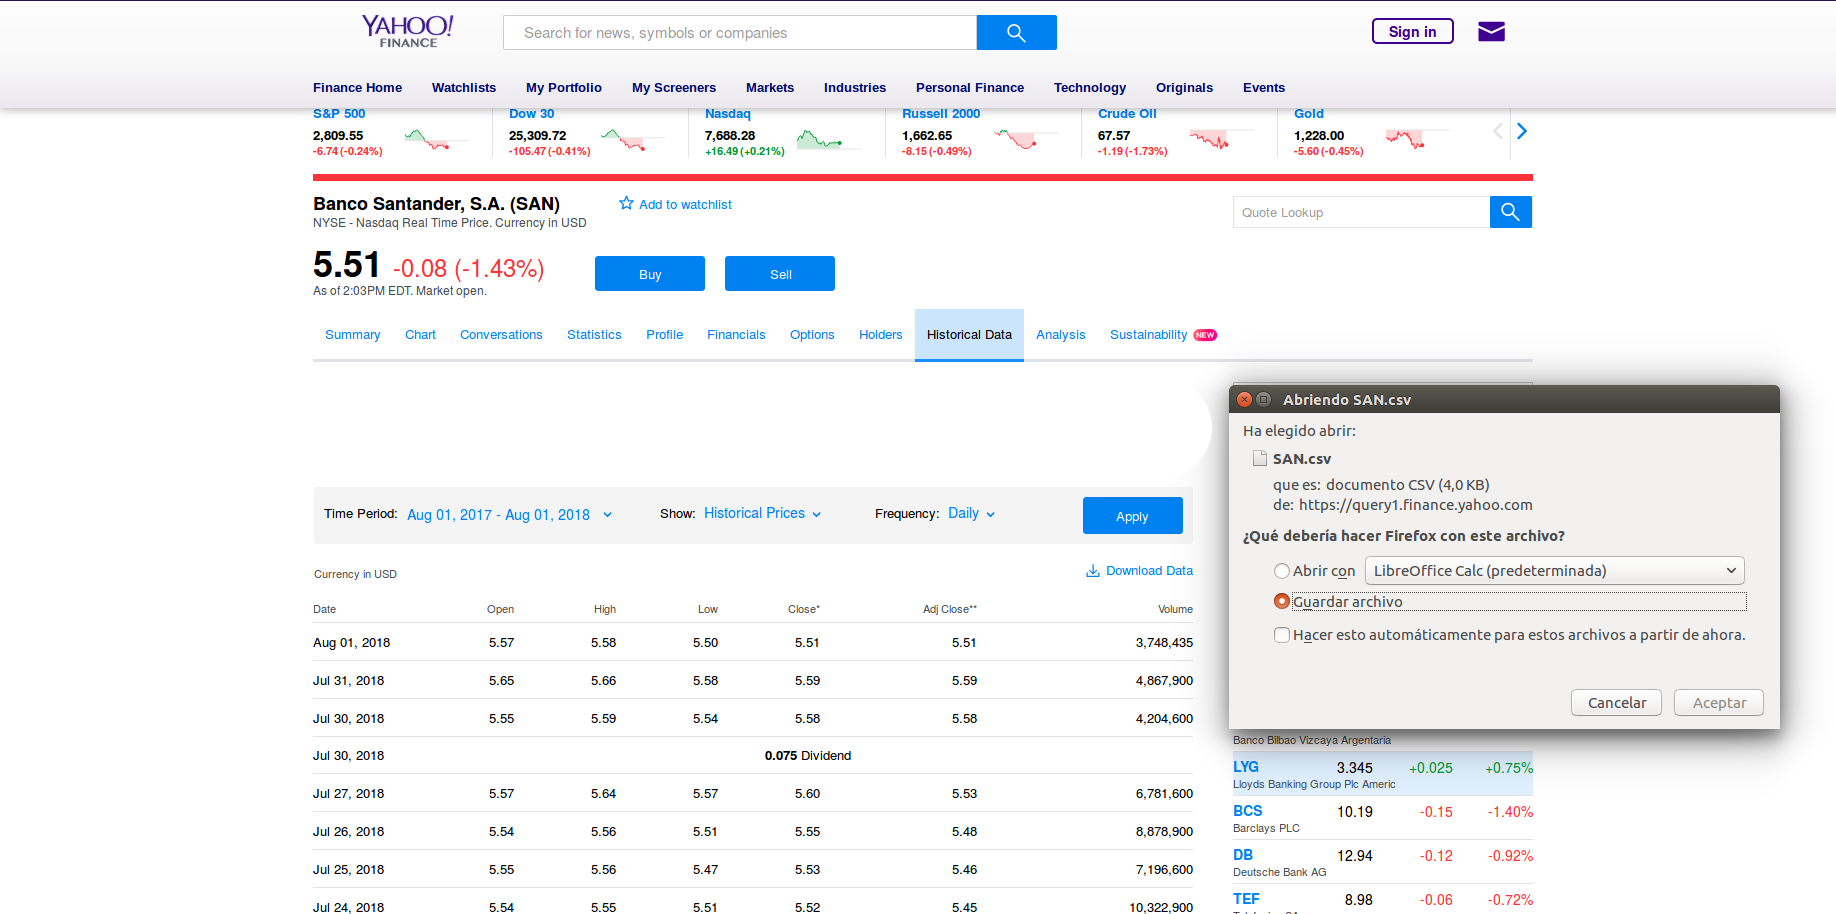
\includegraphics[scale=1]{imagenes/yahoo_finance.png}
			\caption[Descarga de los datos hist\'oricos con \textit{Yahoo! Finance}]{Descarga de los datos hist\'oricos de \textit{Banco Santander}. \\ Fuente: elaboraci\'on propia.}
			\label{fig:yahoo_finance}
		\end{figure}
				
		Por ejemplo, imaginemos que buscamos los valores hist\'oricos de \textit{Banco Santander} desde el 1 de agosto de 2017 hasta la misma fecha del a\~{n}o siguiente. Para ello indicamos la empresa, buscamos el apartado de \textit{Historical Data} e indicamos las fechas. El resultado se muestra en la figura \ref{fig:yahoo_finance}.\\
		
		Finalmente, para cargar estos datos en \textit{backtrader} basta con indicar la ruta donde se encuentra el archivo en el ordenador y el rango de fechas que se quiere ejecutar con el siguiente c\'odigo:\\
		

		\begin{lstlisting}[basicstyle=\tiny]
   # Crear un paquete de datos con YAHOO FINANCE
   data = bt.feeds.YahooFinanceCSVData(
	   dataname='Data/SAN.csv',
	   fromdate=datetime.datetime(2017, 8, 1),
	   todate=datetime.datetime(2018, 8, 1),
	   reverse=False)
   
   # Activar los datos en el cerebro
   cerebro.adddata(data)
		\end{lstlisting}

		Aunque en principio carece de inter\'es, el rango de fechas que se indique debe estar contenido en el archivo, pero no tiene por qu\'e ser el mismo. Este hecho permite descargar y almacenar grandes cantidades de datos, previo a su uso, y almacenarlas para un futuro.\\
		
		Esta opci\'on para adquirir datos es sencilla al tener interfaz gr\'afica, pero no se recomienda si se requiere ejecutar muchas veces con distintas empresas. Por tanto, queda descartado su uso por el momento.\\


    \subsubsection{Pandas Datareader}
    De forma alternativa a la descarga de CSV anterior, podemos utilizar el paquete \textit{Pandas-datareader}, que proporciona una funci\'on que automatiza la descarga de datos de \textit{YAHOO! Finance}.\\ 
    
    Aunque estuvo un tiempo en desuso y en su documentaci\'on est\'a marcado as\'i\footnote{\url{https://pandas-datareader.readthedocs.io/en/stable/whatsnew.html\#v0-6-0-january-24-2018} [\'Ultima consulta 20 de Julio de 2019]}, ahora vuelve a estar operativo. La \textit{API} de \textit{YAHOO! Finance} cambi\'o y, durante un tiempo, \textit{Pandas-datareader} no la actualiz\'o. No obstante, el tratamiento de los datos por parte de \textit{Pandas-datareader} ya se ha adaptado, aunque no se vea reflejado a\'un en su documentaci\'on.\\
    
    Por nuestra parte, porcomodidad, usaremos a partir de ahora la siguiente f\'ormula para cargar los datos en \textit{Backtrader}:\\
    
    \begin{lstlisting}[basicstyle=\tiny]
    start_date = "2013-08-01"
    end_date   = "2014-02-26"
    simudatos = pdr.get_data_yahoo("SAN", start=start_date, end=end_date)
    df_cerebro = bt.feeds.PandasData(dataname = simudatos)
    \end{lstlisting}
    
    Como puede observarse en el c\'odigo, basta llamar a la funci\'on con el s\'imbolo de la empresa y las fechas de inicio y fin para descargar los datos diarios. N\'otese que la descarga se realiza desde el propio script y es necesaria realizarla en cada ejecuci\'on, pero se hace de forma autom\'atica. Aunque suponga una peque\~na carga para el tiempo, lo usaremos por la  facilidad de cambiar de fechas y empresa.\\
    
\newpage
\section{Algoritmos gen\'eticos}\label{sec:genetico}
		La evoluci\'on es un proceso de optimizaci\'on cuyo objetivo es la mejora continua de una habilidad o caracter\'istica. Este proceso se observa en la mayor\'ia de los seres vivos que, en un intento de adaptarse al medio y fortalecerse, cambian progresivamente.\\
		
		Los algoritmos gen\'eticos tienen como inspiraci\'on este comportamiento. Para hallar la soluci\'on \'optima de un problema, se genera una poblaci\'on de soluciones, no necesariamente buenas. A continuaci\'on, se simula una descendencia de estas, es decir, nuevas soluciones del problema que se parecen a las anteriores y, mediante selecci\'on natural, se favorece la evoluci\'on de las soluciones hacia una mejora. En el caso de los algoritmos gen\'eticos, esta selecci\'on natural requiere de una forma de medir la bondad de una soluci\'on. Si se reitera este proceso la poblaci\'on de soluciones ir\'a potenciando la caracter\'istica que consigue mejor puntuaci\'on en la manera de medir.\\ 
		
		A continuaci\'on se ofrece una aproximaci\'on a los algortimos gen\'eticos. Un desarrollo m\'as profundo puede encontrarse en otras obras\footnote{Engelbrecht, A. P. (2007). \textit{Computational intelligence: an introduction}. John Wiley \& Sons.  }.
		
		\subsection{Definici\'on}
		Un algoritmo gen\'etico es un conjunto de procedimientos ordenados que, efectuados de forma iterativa y aplicados sobre un conjunto de posibles soluciones, hacen mejorar a la agrupaci\'on hacia unas soluciones mejores. Se identifican cinco elementos b\'asicos en un algoritmo gen\'etico:\\
		
		\begin{itemize}
			\item \textbf{Poblaci\'on.} Es un conjunto de soluciones del problema que queremos resolver, cuya representaci\'on computacional definir\'a al resto de los elementos.
			\item \textbf{Funci\'on \textit{fitness} o funci\'on de evaluaci\'on.} Es la funci\'on cuyo dominio es la poblaci\'on del problema y que tiene por imagen alg\'un subconjunto de ${\rm I\!R}$. Esta funci\'on, hablando en t\'erminos matem\'aticos, es una norma que eval\'ua c\'omo de buena es una soluci\'on.
			\item \textbf{Cruce.} Es un proceso mediante el cual varias soluciones producen una o varias soluciones combinadas nuevas. 
			\item \textbf{Mutaci\'on} Se define como el proceso que act\'ua sobre un individuo de la poblaci\'on y le produce una transformaci\'on signficativa. Este procedimiento no es imprescindible, pero ayuda a que las soluciones sigan variando tras muchas generaciones.
			\item \textbf{Selecci\'on.} Es el criterio de eliminaci\'on que permite eliminar individuos de la poblaci\'on.
		\end{itemize}
		
		En los siguientes ep\'igrafes se va a profundizar en cada elemento de un algoritmo gen\'etico, mostrando especial inter\'es en ver los valores m\'as usuales de estos.\\
		
			\subsubsection{Poblaci\'on}
			En la naturaleza, cada organismo tiene unas caracter\'isticas concretas que influyen en su habilidad para sobrevivir y reproducirse. Estas caracter\'isticas, en  \'ultima instancia, son definidas por los cromosomas de dicho individuo. En un algoritmo gen\'etico, se usa tradicionalemente la notaci\'on de cromosoma para referirse a la codificaci\'on de un individuo.\\
			
			La representaci\'on cl\'asica de un cromosoma es un vector de \textit{bits} de dimensi\'on fija. \\
			
			En el caso de que el espacio de b\'usqueda sea discreto, cada individuo de la poblaci\'on se puede representar con un vector de longitud $n$ donde $2^n$ es el n\'umero de valores posibles del espacio.\\
			
			En el caso continuo, tomaremos ${\mathbb{R}^n}$ como espacio de b\'usqueda y ser\'a necesario acotarlo, es decir, el dominio adopta la forma \\
			\[[x_{min_1}, x_{max_1}]\times\dots\times[x_{min_i},x_{max_i}]\times\dots\times[x_{min_n},x_{max_n}]\]
			
			Entonces, mediante una representaci\'on binaria, por ejemplo la de coma flotante de longitud $l$, podemos transformar cada $x=(x_1,\dots,x_i,\dots,x_n) \in \mathbb{R}^n$ del dominio en $b=(b_1,\dots,b_i,\dots,b_n)$ donde $\forall  0<i\leq n$ $b_i \in \{0,1\}^l$. Es decir, se traslada el espacio continuo a una aproximaci\'on en coma flotante. N\'otese que la precisi\'on num\'erica de un computador siempre es finita y, por tanto, ninguna representaci\'on puede cubrir el espacio de b\'usqueda continuo al completo. No obstante, Esta aproximaci\'on nos permite trabajar con el caso continuo igual que con el caso discreto con buenos resultados.\\
			
			Por supuesto, lo anterior es solo una propuesta cl\'asica que se aplica a un caso gen\'erico. Seg\'un el problema a tratar, un individuo puede ser representado de otras formas m\'as convenientes.\\
			
			Una vez que tenemos definida la estructura de un individuo, la poblaci\'on ser\'a un conjunto de estos. La cantidad de individuos de la poblaci\'on se puede variar a lo largo de la ejecuci\'on del algoritmo, aunque, cuanto mayor sea el n\'umero de individuos, mayor ser\'a el espacio de b\'usqueda inspeccionado y mejores ser\'an los resultados. Eso si, cuanto m\'as exaustiva sea la b\'usqueda, mayor ser\'a el tiempo de ejecuci\'on.\\
			
			Otro factor importante a tratar es la calidad de la poblaci\'on en la primera generaci\'on, ya que esta determinar\'a, en gran medida, la calidad de las generaciones posteriores. En el caso de que no se tenga informaci\'on previa sobre el problema se puede optar por tomar una poblaci\'on inicial aleatoria. No obstante, contruir una poblaci\'on inicial cercana a la soluci\'on acelera el proceso de convergencia. \\
				
			\subsubsection{Funci\'on \textit{fitness}}
			En un modelo evolutivo, el individuo con mejores caracter\'isticas tiene mayores posibilidades de sobrevivir. Para valorar cu\'an bueno es un individuo de la poblaci\'on, se necesita una funci\'on matem\'atica que cuantifique la bondad de este. Definimos la funci\'on \textit{fitness} o funci\'on de evaluaci\'on como 
			\[f:\Gamma\rightarrow\mathbb{R}\]
			donde $\Gamma$ es el espacio en el que se definen los individuos de la poblaci\'on.\\
			
			Esta funci\'on debe evaluar cada individuo de cada generaci\'on. Luego, al tratarse de un algoritmo iterativo, conviene que la funci\'on no sea computacionalmente pesada. A menudo se usan aproximaciones de la funci\'on de evaluaci\'on real con el fin de ahorrar tiempo.\\
		
			\subsubsection{Selecci\'on}
			La selecci\'on es el operador b\'asico de la evoluci\'on. Su objetivo es dar importancia a los individuos fuertes y aumentar su presencia. Se pueden aplicar operadores de selecci\'on en dos momentos a lo largo del algoritmo:\\
			
			\begin{itemize}
				\item En la selecci\'on de la nueva generaci\'on, con el objetivo de filtrar los individuos m\'as fuertes (los mejor valorados hablando en t\'erminos de la funci\'on \textit{fitness}).
				\item En el cruce de los individuos, con el fin de producir una nueva generaci\'on. Es razonable que los individuos con mejores caracter\'isticas tengan m\'as posibilidades de tener descendientes en la pr\'oxima generaci\'on.
			\end{itemize}
			
			\hspace{0.25cm}Existen multitud de formas de aplicar la selecci\'on, las m\'as comunes son las siguientes:\\
			
			\textbf{Selecci\'on aleatoria}
			
			Cada individuo de la poblaci\'on tiene la misma probabilidad de salir elegido, $\frac{1}{s}$, donde $s$ es el n\'umero de individuos. Siguiendo una distribuci\'on uniforme en $[0,1]$ se pueden extraer los individuos.\\
			
			\textbf{Selecci\'on proporcional}
			
			La probabilidad de que un individuo sea seleccionado viene dado por la funci\'on $\varphi:\Gamma\rightarrow [0,1]$, definida como
			\[\varphi(x_i)=\frac{f(x_i)}{\sum\limits_{j=1}^{s}f(x_j)}\]
			
			Esto es, cada individuo tiene una probabilidad de ser seleccionado proporcional a la valoraci\'on de la funci\'on \textit{fitness}.\\
			
			Al igual que en la selecci\'on anterior, una distribuci\'on uniforme se puede usar para extraer individuos.\\
			
			\textbf{Selecci\'on por torneo}
			
			Se extrae una muestra, con o sin devoluci\'on, de la poblaci\'on de tama\~no $k$ con $k<s$. De entre estos, se selecciona el individuo con mayor puntuaci\'on en la funci\'on \textit{fitness}.\\
			
			El proceso se repite hasta que se hayan extraido todos los individuos requeridos.\\
			
			\textbf{Selecci\'on basada en posición}
			
			En lugar de usar directamente la puntuaci\'on de la funci\'on \textit{fitness}, se usa la posici\'on respecto al resto de individuos de la poblaci\'on.\\
			
			Por tanto, se selecciona el elemento $x_i$ donde $i=Entera(Z)$ y $Z\sim U(0,U(0,s))$, siendo U la distribuci\'on uniforme.\\
			
			\textbf{Selecci\'on con elitismo}
			
			En ciertos casos conviene mantener a los mejores individuos de una poblaci\'on, lo que permitir\'a asegurar que la nueva poblaci\'on tendr\'a alg\'un individuo, al menos, tan bueno como el mejor de la generaci\'on anterior.\\
			
			Seleccionar varios individuos para que permanezcan en la poblaci\'on suele ser una buena pr\'actica.\\
			
			\subsubsection{Cruce}
			
			La reproducci\'on es el proceso mediante el cual los individuos de una poblaci\'on dan lugar a la siguiente poblaci\'on. As\'i pues, un cruce es una operaci\'on que, dados uno o varios individuos padres, genera uno o varios individuos hijos que ser\'an parte de la pr\'oxima generaci\'on.\\
			
			La forma t\'ecnica de hacer un cruce depende directamente de la representaci\'on de los individuos. Por tanto, dado que fue el caso descrito anteriormente, vamos a presentar algunas formas de hacer cruces cuando tenemos representaci\'on binaria.\\
			
			\textbf{Cruce de un punto}
			
			Dados dos padres a cruzar, se toma un valor $i$ donde $i=Entera(Z)$ y $Z\sim U(1,l-1)$ con $l$ la longitud del vector de \textit{bits} que representa a un individuo. \\
			
			En consecuencia se crean dos nuevos individuos. El primero tendr\'a los $i$ primeros \textit{bits} del primer padre y los $l-i$ \'ultimos del segundo progenitor. El segundo individuo, por su parte, se genera con los bits que no se han tomado en el primero.\\
			
			\textbf{Cruce de dos puntos}

			Este cruce es similar al anterior, con la diferencia de que la parte que se toma del primer padre para el primer hijo viene dada por una subcadena, de los \textit{bits} del padre, que comienza y acaba en dos \'indices generados con una distribuci\'on uniforme, tal y como venimos haciendo.\\
			
			N\'otese que aleatorizar el final de la subcadena es equivalente a aleatorizar la dimensi\'on de la misma. En ocasiones se puede optar por una subcadena de tama\~no fijo. \\
			
			\textbf{Cruce uniforme}
			
			Es un procedimiento similar a los anteriores, solo que el reparto se hace \textit{bit} a \textit{bit}. Se inicializa una m\'ascara de tama\~no $l$ con los \textit{bits} a 0. Por cada elemento de la m\'ascara, se toma un valor de $X \sim U(0,1)$; si $x > p$, entonces el valor de la m\'ascara se actualiza a 1. El primer hijo tendr\'a los bits del primer padre que tengan 0 en la m\'ascara y el resto del segundo padre. Por su parte, el segundo hijo se construye de forma contraria. \\
			
			
			\subsubsection{Mutaci\'on}

			El objetivo de las mutaciones es la introducci\'on de nuevo material gen\'etico en la poblaci\'on, m\'as all\'a de las combinaciones entre los individuos. Una mutaci\'on demasiado frecuente o demasiado agresiva producir\'a que se pierda el factor evolutivo, no obstante, en aplicado en determinadas dosis puede llegar a ser efectivo si se desea explorar m\'as en el espacio de b\'usqueda.\\
			
			Del mismo modo que en la secci\'on de cruce, tenemos distintas variantes de esta operaci\'on basadas en la forma de escoger los bits a mutar.\\
			
			Una vez m\'as, las distintas variantes est\'an basadas en la representaci\'on binaria. Otras representaciones de los individuos necesitan de otras mutaciones adaptadas al caso correspondiente.\\
			
			\textbf{Mutaci\'on uniforme}

			En este caso, dado un individuo, se seleccionan, a partir de una distribuci\'on uniforme, los \textit{bits} que se van a mutar. La mutaci\'on consiste, pues, en alterar cada posici\'on con el valor contrario al original (0 si era 1 y 1 si era 0).\\			
		
		
			\textbf{Mutaci\'on \textit{inorder}}
		
			Es un caso similar al anterior, pero los \textit{bits} mutables son solo un subconjunto de los totales. Dicho subconjunto inmutable puede ser producto de una aleatorizaci\'on o, simplemente, ser seleccionado manualmente si se quiere proteger una zona de la representaci\'on de este operador.\\
			

			\textbf{Mutaci\'on Gaussiana}

			Esta es una mutaci\'on basada en el m\'etodo de ruido Gaussiano. Si se ha usado la codificaci\'on binaria de los individuos, es necesario volver al valor decimal que este representa, por lo que solo es v\'alida en espacios de b\'usqueda continuos.\\
			
			Una vez se tiene el valor decimal, se usa el m\'etodo de ruido Gaussiano sobre el valor, esto es, $x_j = x_j + N(0,\sigma_j)$, con $N$ la distribuci\'on normal y $\sigma_j = x_j * 0.1$\\
			
			Finalmente, para concluir se devuelve la variable a la codificaci\'on binaria.\\
			
			Con este \'ultimo m\'etodo se pueden proteger los cambios dr\'asticos en los valores, ya que la distribuci\'on normal controla que no se cambien los \textit{bits} m\'as significativos en la codificaci\'on binaria.\\
			
			Enti\'endase que en un marco pr\'actico, los valores son decimales pero se guardan en la m\'aquina con representaci\'on binaria. Luego las transformaciones entre binaria y decimal se hacen de forma sistem\'atica. Adem\'as, al generar un valor con la distribuci\'on normal, \'este ya est\'a en representaci\'on binaria.\\ 
							
		\subsection{Ejemplo de algoritmo gen\'etico con \textit{Pyvolution}}
		
		\textit{Pyvolution} es un paquete de \textit{Python} que facilita el uso de algoritmos gen\'eticos. Aunque la \'ultima versi\'on fue lanzada en 2012, es un paquete completo, con una sintaxis simple y sencillo de utilizar. En apenas 30 lineas y sin necesidad de dar muchas especificaciones, se pueden realizar algoritmos completos. Una ejecuci\'on normal consta de varios par\'ametros, a trav\'es de los cuales se pueden controlar las caracter\'isticas de las generaciones, los individuos por generaci\'on, probabilidad y severidad de las mutaciones, cantidad de individuos elitistas e, incluso, el tiempo m\'aximo de ejecuci\'on.\\
		
		Para ilustrar brevemente su uso, se adjunta uno de los ejemplos que vienen en la p\'agina de \textit{Github} del paquete.\footnote{\url{https://github.com/littley/pyvolution} [\'Ultima consulta 10 de Julio de 2019]}\\
		
		\begin{lstlisting}[basicstyle=\tiny]
	import math
	from pyvolution.EvolutionManager import *
	from pyvolution.GeneLibrary import *
	
	"""
	Queremos calcular una solucion del siguiente sistema:
	a + b + c - 17 = 0
	a^2 + b^2 - 5 = 0
	"""
		
	def fitnessFunction(chromosome):
		"""
		Dado un "cromosoma", esta es la funcion que calcula su puntuacion
		La puntuacion es una float mayor que 0.
		"""
		
		#Accedemos a los cromosomas o valores a ajustar
		a = chromosome["a"]
		b = chromosome["b"]
		c = chromosome["c"]
		d = chromosome["d"]
		
		#Calculamos los valores que nos gustaria que fueran 0
		val1 = math.fabs(a + b + c - 17)
		val2 = math.fabs(math.pow(a, 2) + math.pow(b, 2) - 5)
		
		#La funcion distancia agrupa los valores para una mejor puntuacion
		dist = math.sqrt(math.pow(val1, 2) + math.pow(val2, 2)
		
		if dist != 0:
		return 1 / dist # Cuanto menor sea la distancia mayor sera la puntuacion
		else:
		return None     #Devolver None indica que los cromosomas han sido ajustados
		
		
	#Configuramos el algoritmo genetico
	em = EvolutionManager(
		fitnessFunction,
		individualsPerGeneration=100,
		mutationRate=0.2,	#Probabilidad de mutacion
		maxGenerations=1000,
		stopAfterTime=10,   #Para simulacion tras 10 segundos
		elitism=2,          #Mantener los 2 mejores de cada generacion
	)
		
	#Creamos una funcion de mutacion inversamente proporcional a la bondad del ajuste
	mutator = FloatInverseFit("mut", maxVal=0.01, startVal=1)
		
	#Indicamos que los puntos iniciales se toman siguiendo una distribucion normal
	#de media 0 y desviacion 100. Ademas marcamos la mutacion como la definida antes.
	atype = FloatGeneType("a", generatorAverage=0, generatorSTDEV=100, mutatorGene="mut")
	btype = FloatGeneType("b", generatorAverage=0, generatorSTDEV=100, mutatorGene="mut")
	ctype = FloatGeneType("c", generatorAverage=0, generatorSTDEV=100, mutatorGene="mut")
		
	#Registramos los parametos y la mutacion
	em.addGeneType(mutator)
	em.addGeneType(atype)
	em.addGeneType(btype)
	em.addGeneType(ctype)
	
	#Ejecutamos	
	result = em.run()
		\end{lstlisting}

    A pesar de la sencillez, no es pr\'actico usar este paquete de \textit{Python} para nuestro prop\'osito. Los \'arboles que van a componer nuestra poblaci\'on tienen muchas variables que deben ser introducidas en la herramienta gen\'etica. Adem\'as, algunas de las variables son continuas, como los par\'ametros de algunos indicadores, y otras variables son discretas, como el indicador de cada nodo.\\
    
    As\'i mismo, \textit{backtrader} tiene posibilidad de paralelizaci\'on en la ejecuci\'on. Esto permite que la funci\'on \textit{fitness}, el factor que m\'as incapacita computacionalmente, se pueda ejecutar mucho m\'as r\'apido.\\
    
    No obstante, el problema que descarta definitivamente este paquete es la imposibilidad de hacer cruces entre \'arboles. Solo est\'a preparado para trabajar con representaciones num\'ericas.\\
    
    En lugar de usar \textit{Pyvolution}, realizaremos una estructura de algoritmo gen\'etico propio. Esto llevar\'a m\'as trabajo, pero se obtendr\'a un algoritmo m\'as r\'apido.\\
\newpage
\section{\'Arbol de Decisi\'on}\label{sec:Decision_tree}
	
		Los \'arboles se utilizan en diversos campos de la inform\'atica. A pesar de que son dif\'iciles de representar y visualizar de forma global, resultan una herramienta muy \'util para separar situaciones o datos.\\
		
		La estructura de los \'arboles se puede usar con muchos fines: ordenar un vector, resolver problemas de alta complejidad computacional (como encontrar la mejor jugada posible en un tablero de ajedrez), representar redes de routers y switches o expresar la gram\'atica de un lenguaje, entre otros.\\
		
		En el caso que nos ocupa, estamos interesados en un tipo muy especial de \'arboles, los \'arboles de decisi\'on.\\
		
		\subsection{Definici\'on}
			Un grafo es un conjunto de v\'ertices y aristas. Las aristas tienen dos extremos, en cada uno de ellos se sit\'ua un v\'ertice.\\
			
			Un grafo simple es aquel que no tiene lazos (aristas cuyos extremos se conectan con el mismo v\'ertice) ni aristas m\'ultiples entre dos de sus v\'ertices.\\
			
			Un \'arbol es, pues, un grafo simple tal que
			para cada dos v\'ertices de existe un \'unico camino simple entre ellos, es decir, hay una \'unica sucesi\'on de aristas que empieza en uno de los v\'ertices y termina en el otro sin repetir arista.\\
			
			Un \'arbol de decisi\'on ser\'a, por tanto, una especializaci\'on de \'arbol en la que a los v\'ertices se los interpreta de la siguiente forma:\\
			
			\begin{itemize}
				\item Un v\'ertice especial, llamado nodo ra\'iz, se considera el inicio del camino de decisi\'on.
				\item Un conjunto de v\'ertices, llamados nodos, se conectan con, al menos, otros dos v\'ertices. En cada nodo hay una condici\'on. La verficaci\'on de dicha condici\'on determina qu\'e nodo es el siguiente en el camino de decisi\'on.
				\item Un conjunto de v\'ertices, llamados hojas o nodos terminales, se conectan con un \'unico v\'ertice. En cada hoja hay una clasificaci\'on del dato que cumple todas las condiciones que tienen los nodos del camino que empieza en la ra\'iz y termina en la hoja. 
			\end{itemize}
			
			El objetivo de un \'arbol de decisi\'on es, por tanto, clasificar datos, de una determinada naturaleza, seg\'un una serie de condiciones. La construcci\'on de dicho \'arbol y la elecci\'on de las condiciones las veremos en los siguientes apartados.\\
		
			En este punto, se procede a plantear un problema cl\'asico para dar un ejemplo de \'arbol de decisi\'on. En un campeonato de tenis al aire libre son necesarias unas buenas condiciones metereol\'ogicas. Para tomar la decisi\'on de si se puede jugar un partido, o no, se puede utilizar el \'arbol de decisi\'on de la figura \ref{fig:tenis}.
			
			\begin{figure}[H]
    			\centering
    			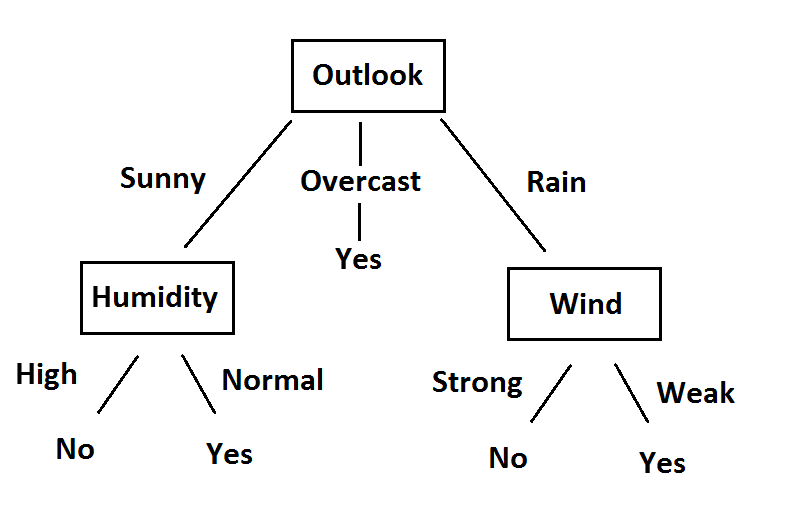
\includegraphics[scale=0.5]{imagenes/tree.png}
    			\caption[\'Arbol de decisi\'on para jugar partido de tenis.]{\'Arbol de decisi\'on para decidir si un partido de tenis se juega.\\ Fuente: \url{https://sefiks.com} [\'Ultima consulta 12 de Julio de 2019]}
    			\label{fig:tenis}
		    \end{figure}
			
			Como se puede ver, el \'arbol se interpreta del nodo ra\'iz hasta las hojas. Luego la primera condici\'on a comprobar es el estado del cielo: si est\'a nublado, entonces se juega; si por el contrario, est\'a soleado o lloviendo, entonces hay que comprobar otra condici\'on para tomar la decisi\'on.\\
			
			En este ejemplo es clara la identificaci\'on de los elementos del \'arbol de decisi\'on. La clasificaci\'on de los partidos se compone de dos etiquetas: s\'i se puede jugar y no es factible jugar. Del mismo modo, las condiciones presentes en el \'arbol son tres:\\
			
			\begin{itemize}
				\item \textbf{Situaci\'on del cielo.} Puede tomar tres valores; soleado, nublado y lluvioso.
				
				\item \textbf{Humedad.} Condici\'on que puede tomar dos valores; humedad alta y humedad normal.
				
				\item \textbf{Viento.} Puede tomar dos valores; viento fuerte o viento d\'ebil.
			\end{itemize}
		
			En los siguientes ep\'igrafes se desarrollar\'a c\'omo se pueden construir estos \'arboles de forma met\'odica.\\
			 
			\subsubsection{Etiquetado}
			Para poder clasificar un dato, es necesario saber cu\'ales son las posibles clasificaciones o, dicho de otra manera, cu\'ales son las clases de los datos. Esta clase viene dada por la etiqueta o \textit{tag}. En el ejemplo anterior del campeonato de tenis las clases ser\'ian jugar y no jugar.\\
			
			Cuando el problema solo tiene dos clases se denomina problema binario. Aunque son los problemas m\'as comunes, en algunas ocasiones puede interesar discutir entre m\'as clasificaciones. Por ejemplo, se puede construir un \'arbol de decisi\'on que clasifique todos los delitos de c\'odigo penal atendiendo a la dureza de su pena: baja, media o alta.\\
			
			En el caso que nos ocupa, el \textit{trading} en bolsa, no se tiene una clasificaci\'on natural para los valores de las acciones. Es claro, seg\'un el objetivo adelantado en la introducci\'on, que se tiene que diferenciar entre los instantes buenos para comprar y aquellos que son buenos para vender. Pero, la definici\'on de qu\'e es un buen d\'ia para comprar no es clara. \\
			
			En principio, parece buena la idea de clasificar como d\'ias de compra aquellos en los que el precio de la acci\'on, tras un periodo razonable, sube. De forma an\'aloga, los d\'ias de venta son aquellos a partir de los cuales el precio de la acci\'on baja. \\
			
			Crear estas clases de manera que representen un buen momento para comprar o vender es objeto de estudio en nuestro trabajo, pero por motivos de secuenciaci\'on, se hablar\'a de ello m\'as tarde.\\
			
			\subsubsection{Conjunto de entrenamiento}
			Una vez que la estructura del \'arbol est\'a hecha, es sencillo clasificar un dato. Basta con ir comprobando las condiciones de cada nodo y continuar el recorrido del grafo, seg\'un los resultados de estas. Cuando una condici\'on nos dirija a una hoja, encontraremos la clase predicha para ese dato concreto. Pero, ¿c\'omo podemos crear el \'arbol?\\
			
			Aqu\'i entra en juego el conjunto de entrenamiento. Un conjunto de entrenamiento es un compendio de datos de la misma naturaleza que los que queremos clasificar, pero que ya est\'an clasificados. La forma de dar una categor\'ia a estos datos de forma previa a tener el \'arbol es muy variada. No obstante, la mejor opci\'on suele ser contar con el conocimiento experto de alguien capaz de clasificar los datos.\\
			
			Por tanto, a partir de este conjunto etiquetado, deberemos inducir un \'arbol de decisi\'on cuyas hojas clasifiquen bien los datos conocidos. Se han propuesto, en distintos manuales, diferentes formas de construirlos. Si se desea profundizar m\'as en estas construcciones se puede consultar Barros (2015), aqu\'i no se desarrollar\'an.\\
			
			De esta forma, si los datos con clase desconocida tienen una procedencia parecida a los datos del conjunto de entrenamiento, ser\'an correctamente clasificados por el \'arbol construido con los datos de clase conocida. O, al menos, esta es la intenci\'on.\\
			
			Los \'arboles de decisi\'on tambi\'en se pueden formar a partir de otros m\'etodos, por ejemplo, a partir de conocimiento de una procedencia segura. En nuestra propuesta, lo haremos a partir de un algoritmo gen\'etico.\\
	
\newpage
\section{Algoritmo propuesto}\label{sec:algorithm}

En este proyecto de fin de grado, se propone un algoritmo gen\'etico basado en \'arboles de decisi\'on cuyo objetivo es extraer informaci\'on de se\~nales de compra. Es decir, se pretende dise\~nar un \'arbol de decisi\'on que sirva como modelo para saber cu\'al es el momento id\'oneo para situar \'ordenes de compra y de venta en el mercado de valores y extraer beneficio.\\

\subsection{\'Arboles de decisi\'on}
El primer punto a tratar para dise\~nar el modelo, que se va  utilizar para extraer las se\~nales de compra y venta, es la estructura del \'arbol de decisi\'on. En primer lugar se expone la elecci\'on de las etiquetas. A continuaci\'on, se desarrollar\'a el contenido de los nodos, en otras palabras, las condiciones que dividen los caminos.\\

En cuanto a la clasificaci\'on de los d\'ias de bolsa, se propone un dise\~no con tres etiquetas:
\begin{itemize}
    \item Etiqueta \textit{Buy}. Un d\'ia clasificado con esta etiqueta, es un d\'ia bueno para comprar. Implica que el modelo env\'ia una se\~nal de compra y, consecuentemente, se debe colocar una orden de compra de acciones, tantas como nos sea posible con el capital disponible.
    \item Etiqueta \textit{Sell}. En el caso de que un d\'ia se clasifique con esta, signfica que es un buen d\'ia para vender. Implica que el modelo env\'ia una se\~nal de venta y, por tanto, se ha de colocar una orden de venta de todas las acciones que se tengan.
    \item Etiqueta \textit{Stop}. Es una etiqueta comod\'in que se usa cuando las condiciones de un camino no son concluyentes para decidir si hay que comprar o vender. En esta situaci\'on el modelo no env\'ia ninguna se\~nal.
\end{itemize}

Esta elecci\'on est\'a motivada por la necesidad de que el modelo sea capaz de transmitir se\~nales de compra y venta. La forma m\'as sencilla de conseguir estos env\'ios es utilizar dos etiquetas, una de compra y otra de venta. Pero, de ser as\'i, todos los caminos de condiciones llevar\'ian al modelo a una compra o a una venta. En ciertas ocasiones, el estado de la bolsa puede no ser determinante para decidir si es un momento de compra o de venta. Es entonces cuando aparece, de forma l\'ogica, la tercer etiqueta, ni es momento de comprar ni lo es de vender. \\

Una vez conocida la posible clasificaci\'on, se debe desarrollar cu\'ales van a ser las caracter\'isticas que van a definir la clase de un d\'ia. En otras palabras, es necesario conocer las condiciones que van a constituir los nodos. En el \'arbol se van a situar condiciones que dividen a los nodos en dos ramas, la que cumple la condici\'on y la que no. Por tanto, todos los nodos ser\'an de bifurcaci\'on binaria. Las reglas que se van a evaluar son de la forma: 
 \[indicador(parametros) <= pivote\].
 
 Donde $pivote$ es una un n\'umero real e $indicador$ es eso, un indicador de bolsa, con par\'ametros o no, seg\'un la naturaleza del indicador. Se ha usado la siguiente lista con indicadores cl\'asicos:
 
 \begin{itemize}
     \item MACD
     \item ATR
     \item ROC
     \item EMA
     \item SMA
     \item Momento
     \item HILL
     \item RSI
     \item OBV
     \item AD
     \item TRANGE
     \item BBANDS\_HIGH
     \item BBANDS\_LOW
 \end{itemize}
 
Se adjunta una breve explicaci\'on de cada uno de los indicadores utilizados en el anexo \ref{apendice}.\\ 
 
 En el caso de algunos indicadores, como EMA (\textit{Exponential Moving Average}) o SMA (\textit{Simple Moving Average}), se hace necesaria una ligera modificaci\'on. Esto es debido a que al entrenar un \'arbol en un determinado periodo, en este aparecer\'an reglas como $EMA(10) <= 500$. La potencia del indicador $EMA$ se encuenta al comparar su valor con el valor actual de la acci\'on y observar si se ha producido una bajada o subida importante respecto a los \'ultimos d\'ias.  

 
 		\begin{figure}[H]
    		\centering
    		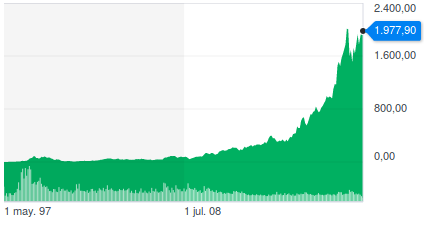
\includegraphics[scale=0.7]{imagenes/amazon.png}
    	    \caption[Valor de las acciones de Amazon en un periodo concreto]{Valor de las acciones de Amazon.\\ Fuente: \url{https://finance.yahoo.com} [\'Ultima consulta 19 de Julio de 2019]}
    		\label{fig:amazon}
	   \end{figure}
	   
En ciertos casos, por ejemplo en tendencias laterales, podr\'ia tener sentido usar esta condici\'on. Si el valor de la acci\'on lleva unos d\'ias demasiado alto o demasiado bajo puede signficar un cambio de tendencia.\\

Pero, en otros casos, resulta fatal. Imaginemos que nuestro modelo aprende en un periodo de entrenamiento en que una condici\'on con $EMA$ es muy significante. Al pasar al periodo de prueba, esta condici\'on puede ser absurda, como en el caso que se ve en la figura \ref{fig:amazon} de Amazon. El valor es solo creciente, no tiene sentido poner un pivote fijo.\\

En su lugar, se propone modificar este indicador restando o dividiendo a su valor el precio actual de la acci\'on para, de alguna forma, escalar el indicador y hacerlo intemporal. En el caso de la divisi\'on, se obtiene la proporci\'on entre el valor actual y un valor representante de los \'ultimos d\'ias. Por su parte, la resta es un poco menos aconsejable, ya que hay una gran diferencia entre que una acci\'on a 2 euros suba 10, y que una acci\'on de 500 euros suba 10. Ambos casos son positivos, pero el primero es mucho m\'as significativo. \\


\subsection{Estructura gen\'etica}
Para construir el \'arbol modelo, se utilizar\'a un patr\'on gen\'etico como el explicado en el apartado \ref{sec:genetico}, en el que, oportunamente, se hizo una explicaci\'on gen\'erica de un algoritmo gen\'etico. A continuaci\'on se procede a replicar esa construcci\'on adapt\'andola a nuestra poblaci\'on, los \'arboles de decisi\'on.\\

En primer lugar, se crea una generaci\'on y, mediante una simulaci\'on de inversi\'on en un periodo de prueba, se puntuan los \'arboles. A continuaci\'on se realiza un proceso de selecci\'on y de cruce de los \'arboles. Y por \'ultimo, se sortea una serie de mutaciones. Una vez terminado el procedimiento, vuelve a comenzar el proceso de simulaci\'on para encontrar la pr\'oxima generaci\'on.\\

A continuaci\'on se va a profundizar en cada uno de los pasos seguidos en este procedimiento.\\

\subsubsection{Primera generaci\'on}
La primera generaci\'on en los algoritmos gen\'eticos suele ser aleatoria y la l\'ogica de los siguientes pasos va perfilando y mejorando la poblaci\'on a largo plazo.\\

Puesto que nuestra simulaci\'on se prev\'e costosa, se va a proceder a realizar un ligero calentamiento de la poblaci\'on para que se reduzcan las iteraciones necesarias hasta la obtenci\'on de una poblaci\'on buena. Con el fin calentar los \'arboles en la primera poblaci\'on, se propone usar una construcci\'on con algunos elementos aleatorios y otros heur\'isticos.\\

En primer lugar, para cada \'arbol se toman indicadores de forma aleatoria que conforman los nodos. Cada vez que se a\~nade un nuevo nodo con su indicador, el pivote que divide los datos se toma a partir de los mejores resultados de una funci\'on de entrop\'ia. La funci\'on de entrop\'ia se aplica sobre los datos del periodo de prueba. A continuaci\'on se explicar\'a detalladamente cada paso. \\

\paragraph{Etiquetado de datos de prueba}
El mismo periodo que se va a usar para entrenar el algoritmo gen\'etico va a ser utilizado para generar esta primera poblaci\'on. As\'i pues, se toman estos datos y se etiquetan siguiendo estas consideraciones:

    Nombremos m\'axima subida, y lo notamos como $M$, a la siguiente expresi\'on:\\
    \begin{align*}
    \begin{split}
        M = \max\limits_{\substack{i,j\in\mathbb{N} \\ i<j}} \{cierre_{j} - cierre_{i} \:|\: \forall z\: con \:i < z\leq j\: cierre_{z-1} - cierre_{z} \geq 0 \}
    \end{split}
    \end{align*}
    
    De forma an\'aloga, se obtiene la m\'axima bajada, notada como m:
    \begin{align*}
    \begin{split}
        m = \max\limits_{\substack{i,j\in\mathbb{N} \\ i<j}} \{cierre_{j} - cierre_{i} \:|\: \forall z\: con \:i < z\leq j\: cierre_{z-1} - cierre_{z} \leq 0 \}
    \end{split}
    \end{align*}

    Seguidamente, se definen dos tipos de tendencias.\\
    
    Una consecuci\'on de d\'ias tiene tendencia positiva siempre que en mitad no se halle una bajada del precio superior a la sexta parte de m.\\
    
    De forma an\'aloga, una consecuci\'on de d\'ias se dice con tendencia negativa si en mitad se halla una subida superior a la sexta parte de M.\\
    
    Es decir,
    
    \begin{align*}
    \begin{split}
        \{i,i+1,...,j\}\: \text{tiene tendencia positiva} \Longleftrightarrow{}\\
        \forall z,k\: con \:i < k < z\leq j\hspace{0.5cm} cierre_{z} - cierre_{k} \geq m/6
    \end{split}
    \end{align*}
    
    \begin{align*}
    \begin{split}
        \{i,i+1,...,j\}\: \text{tiene tendencia negativa} \Longleftrightarrow{}\\
        \forall z,k\: con \:i < k < z\leq j\hspace{0.5cm} cierre_{z} - cierre_{k} \leq M/6
    \end{split}
    \end{align*}

    En \'ultima instancia, se marcan los datos con cuatro etiquetas:
    \begin{itemize}
        \item \textbf{-2} para el \'ultimo d\'ia de cada tendencia negativa.
        \item \textbf{-1} para el resto de d\'ias de las tendencias negativas.
        \item \textbf{2} para el \'ultimo d\'ia de cada tendencia positiva.
        \item \textbf{1} para el resto de d\'ias de las tendencias positivas.
    \end{itemize}
    
    Estas etiquetas son un intento de marcar las diferencias de d\'ias buenos para comprar y d\'ias buenos para vender. \\
    
    En consecuencia, al sumar las etiquetas de un grupo de d\'ias, cuanto m\'as negativo sea el resultado, m\'as influencia tienen los m\'inimos de las tendencias negativas y, por tanto, los d\'ias est\'an orientados a comprar.\\
    
    En el caso contrario, una suma positiva implica una buena fecha para vender.\\
    
    En la figura \ref{fig:tagging} se puede observar un ejemplo simple de etiquetado de un periodo. En ella se ven los tramos clasificados como crecientes en azul y los decrecientes en rojo. Hay que destacar que la transici\'on de $D$ a $E$ es positiva, pero est\'a en mitad de un tramo decreciente y la diferencia no supera la sexta parte de la subida permitida por lo que, seg\'un lo anteriormente expuesto, se marca tambi\'en como decreciente.\\
    
     	\begin{figure}[H]
    		\centering\leftskip=-20px
    		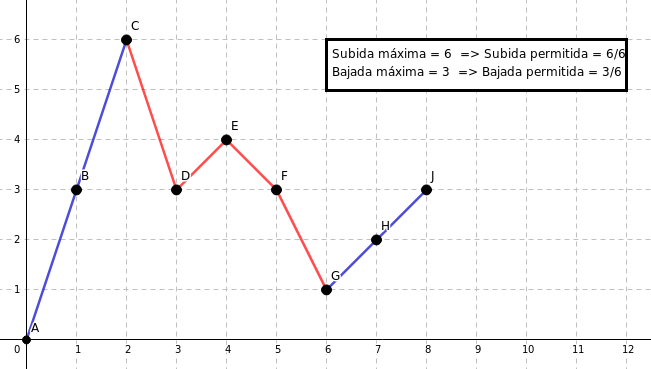
\includegraphics[scale=0.65]{imagenes/tagging.png}
    	    \caption[Ejemplo de etiquetado de un periodo]{Ejemplo de etiquetado de un periodo.\\ Fuente: elaboraci\'on propia}
    		\label{fig:tagging}
	   \end{figure}
    
\paragraph{Selecci\'on de pivotes}
Una vez se ha seleccionado un indicador para el nodo de un \'arbol de la primera generaci\'on, de forma aleatoria, el pivote se selecciona de forma heur\'istica. Hay que destacar que el pivote seleccionado no es el mejor de todos los posibles, simplemente se considera una elecci\'on para rectificar la aleatoridad de la selecci\'on de indicadores.\\

El pivote final elegido es un valor de una rejilla conformada por diez valores equidistantes situados entre el m\'aximo y el m\'inimo valor del par\'ametro de los datos que cumplen las condiciones para llegar al nodo. \\

Puesto que tenemos cuatro etiquetas, en primera instancia se deber\'ia usar una funci\'on de entrop\'ia de cuatro clases. Pero las etiquetas 2 y -2 son poco frecuentes. Adem\'as, debido a que nuestros nodos dividen los datos en dos ramas, no parece oportuno usar una entrop\'ia de cuatro clases. En su lugar proponemos hacer dos clases, una para las etiquetas negativas (-1 y -2), y otra para las positivas (1 y 2).\\

La funci\'on de entrop\'ia de dos clases es, por tanto:\\

$entropy(x) = x*log_{2}(x) + (1-x)log_{2}(1-x) \quad x\in(0,1)$\\

Donde $x$ es la proporci\'on de una de las clases. De este modo, en caso de que la proporci\'on de una clase sea 1, se obtiene la informaci\'on perfecta (la rama solo tiene datos de una clase), pero entonces, la funci\'on entrop\'ia no puede calcularse. Hay que tener en cuenta este caso especial  y evitar realizar el c\'alculo de la funci\'on.\\

Para calcular el mejor pivote de un nodo, se eval\'uan las entrop\'ias de las dos ramas que forma y se hace la suma proporcional al n\'umero de individuos. El pivote cuya funci\'on de entrop\'ia sea mayor es seleccionado como mejor pivote de la rejilla.\\

\paragraph{Selecci\'on de las hojas}
Cuando los datos que cumplen las condiciones de una rama son pocos o la rama ya tiene demasiada profundidad en este calentamiento de la primera generaci\'on, es necesario dar por terminada la rama y culminar la construcci\'on con una hoja.\\

Las hojas son, simplemente, una de las tres se\~nales posibles que permite el modelo propuesto: comprar, vender o no hacer nada.\\

Para escribir la decisi\'on que se debe tomar en esa hoja se va a usar una vez m\'as la etiqueta puesta en los datos de prueba. Notando $x_{tag=a}$ al n\'umero de instancias de los datos que cumplen el camino de condiciones y cuya etiqueta es $a$, definimos la variable que va a determinar la acci\'on de la hoja como:\\

$\alpha = \frac{x_{tag>0}\; -\; x_{tag<0} \; + \; x_{tag=2} \; -\; x_{tag=-2}}{x_{tag>0}\; + \; x_{tag<0}} $\\


Es importante destacar que, para cada hoja, los datos a tratar son aquellos que cumplen las condiciones del camino de nodos hasta la hoja. De este modo, por tanteo se llega a la siguiente adjudicaci\'on de la se\~nal de la hoja:\\

\[   
\text{se\~nal} = 
     \begin{cases}
       \text{Comprar} &\quad\text{si}\quad \alpha < -2\\
       \text{Stop} &\quad\text{si}\quad -2 \leq \alpha \leq 2\\
       \text{Vender} &\quad\text{si}\quad 2 < \alpha\\ 
     \end{cases}
\]

De forma coherente a la se\~nal que se quiere enviar, se colocan las etiquetas.\\

\subsubsection{Cruce}
En cada iteraci\'on del algoritmo se eval\'ua la poblaci\'on con \textit{backtrader} para simular los beneficios que cada individuo tendr\'ia en el periodo de prueba. Una vez extra\'idos los beneficios, se procede a generar la nueva poblaci\'on mediante un cruce que promocione a los \'arboles que mejores resultados han dado.\\

De entre las distintas formas que hay para seleccionar los individuos que se van a reproducir, se escoge la selecci\'on proporcional. M\'as tarde, se explicar\'a el cruce natural de dos \'arboles de decisi\'on\footnote{V\'ease la secci\'on \ref{sec:cruce}}.\\

Este cruce natural entre \'arboles tiene una peque\~na desventaja, y es que puede generar peores poblaciones que las progenitoras. Se hace pr\'acticamente indispensable, entonces, que activemos los m\'etodos elitistas y eliminatorios. Los mejores \'arboles pasar\'an dos veces a la siguiente generaci\'on, una vez mutados y otra vez sin modificar. Por su parte, los peores se descartar\'an por completo tanto del cruce como de la mutaci\'on.\\

\paragraph{Probabilidades de reproducci\'on}
En primer lugar, hay que calcular la probabilidad de cruce de cada individuo. Para ello se hace una normalizaci\'on especial de los beneficios.\\

Restando el beneficio del peor \'arbol a las puntuaciones de todos, se consigue que estas sean siempre mayores o iguales que 0.\\

A continuaci\'on, con el fin de potenciar las estrategias de compra y venta m\'ultiple, m\'as ventajosas que la estrategia de \textit{buy\&hold}\footnote{La estrategia \textit{buy\&hold} es una estrategia cl\'asica que se basa en la compra inicial de todas las acciones posibles y la venta final de las mismas. Esta estrategia recibe su nombre por la l\'ogica que sigue: comprar y mantener.}, se van a modificar ligeramente las ganacias. Por cada venta que produzca un \'arbol, se suma una cantidad fija de euros a sus beneficios. No obstante, para ciertos valores demasiado altos de esta cantidad con los que se supere las comisiones, las compras y ventas se realizar\'an de forma compulsiva. Es importante, por consiguiente, ajustar bien este valor para evitar este resultado.\\

En el \'ultimo paso de la normalizacion, se dividen todas las puntuaciones entre la suma de las puntuaciones. Esto produce que la suma de las mismas sea 1 y, adem\'as, cada valoraci\'on es proporcional a la cantidad de beneficios que reporta, a excepci\'on de la cantidad a\~nadida en favor de las transacciones r\'apidas.\\

Por \'ultimo, tomando $x \sim U[0,1]$ y notando $p_i$ como la puntuaci\'on normalizada del \'arbol i-\'esimo, se pueden sortear los individuos que se reproducen de forma proporcional a su beneficio de la siguiente forma:\\

\[   
seleccionado = 
     \begin{cases}
       \text{\'arbol 1} &\quad\text{si}\quad 0 \leq x < p_1\\
       \text{\'arbol 2} &\quad\text{si}\quad p_1 \leq x < p_1 + p_2\\
       \text{...} \\
       \text{\'arbol n} &\quad\text{si}\quad \sum\limits_{i=1}^{n-1} p_i \leq x \leq \sum\limits_{i=1}^{n} p_i = 1\\ 
     \end{cases}
\]

Son necesarios dos \'arboles para realizar un cruce, del que, a su vez, resultan otros dos \'arboles. Se tienen que ejecutar tantas selecciones como sean necesarias para que la siguiente generaci\'on mantenga el n\'umero de individuos.\\

Una anotaci\'on final es necesaria. En el caso especial de que todos los \'arboles tengan los mismos beneficios, este procedimiento llevar\'ia a dividir por 0. Para evitar esto, de forma natural se divide el intervalo [0,1] en tantos intervalos de igual dimensi\'on como \'arboles haya y continuamos con el caso general. A cada \'arbol se le asigna un intervalo, esta vez, al ser todos iguales, no importa cu\'al y la funci\'on de selecci\'on podr\'ia ser la siguiente:\\

\[   
seleccionado = 
\begin{cases}
\text{\'arbol 1} &\quad\text{si}\quad 0 \leq x < \frac{1}{n}\\
\text{\'arbol 2} &\quad\text{si}\quad \frac{1}{n} \leq x < \frac{2}{n}\\
\text{...} \\
\text{\'arbol n} &\quad\text{si}\quad \frac{n-1}{n} \leq x \leq 1\\ 
\end{cases}
\]



\paragraph{Cruce natural entre dos \'arboles}\label{sec:cruce}
El cruce entre individuos de la poblaci\'on es el mecanismo central de los algoritmos gen\'eticos. En nuestra propuesta, al tener una poblaci\'on de \'arboles, se va a usar el cruce natural entre estos. \\

Como ya se ha introducido en el punto anterior, con este cruce propuesto no se asegura que los \'arboles de una generaci\'on sean mejores que los progenitores. No obstante, entendemos que es una buena forma de agrupar condiciones y de crear asociaciones diferentes de estas. En consecuencia, esto permite explorar el espacio de b\'usqueda de forma que una generaci\'on contenga modelos parecidos para la predicci\'on en bolsa.\\


El cruce parte de dos \'arboles, llamados padres o progenitores. En cada \'arbol progenitor se marca, con un patr\'on aleatorio, un nodo. Es indispensable que dicho nodo no sea una hoja, aunque s\'i podr\'ia ser la ra\'iz. \\

     	\begin{figure}[H]
    		\centering
    		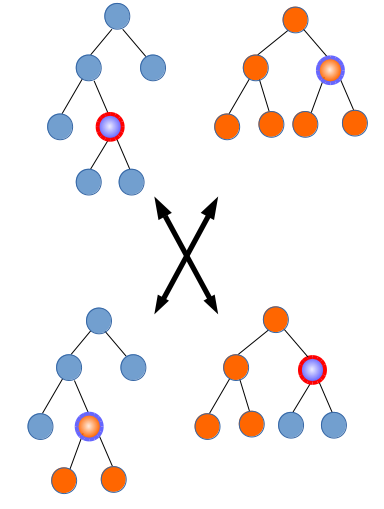
\includegraphics[scale=0.6]{imagenes/crossover.png}
    	    \caption[Ejemplo de cruce entre dos \'arboles]{Ejemplo de cruce entre dos \'arboles.\\ Fuente: elaboraci\'on propia}
    		\label{fig:crossover}
	   \end{figure}

Para construir a los hijos, se intercambian sendos nodos seleccionados y, con ellos, todos los nodos que penden de \'el. En la figura \ref{fig:crossover} puede verse una descripci\'on gr\'afica del cruce.\\

Este cruce puede producir varias anomal\'ias al iterar. Una de ellas es la generaci\'on de \'arboles con una profundidad extrema. Es decir, la poblaci\'on tiene una cierta probabilidad de converger a \'arboles con demasiados nodos o, en su defecto, con insuficientes nodos.\\


     	\begin{figure}[H]
     		\centering
     		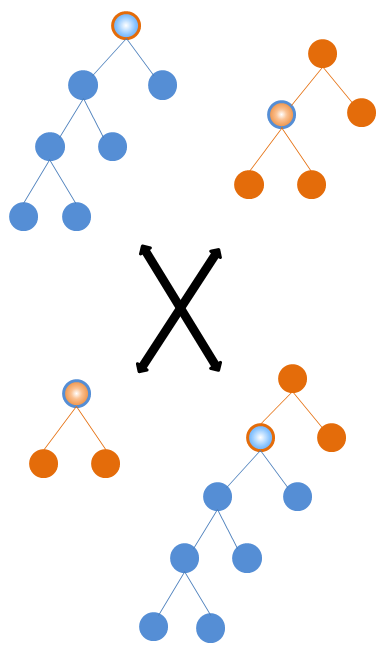
\includegraphics[scale=0.4]{imagenes/small_crossover.png}
     		\caption[Ejemplo de generaci\'on de un \'arbol peque\~no]{Ejemplo de generaci\'on de un \'arbol peque\~no y otro grande.\\ Fuente: elaboraci\'on propia}
     		\label{fig:small_crossover}
     	\end{figure}


Por lo general, un exceso de nodos, que puede entenderse como un exceso de condiciones, va a producir modelos muy espec\'ificos. Los \'arboles demasiado espec\'ificos suelen aprender muy bien la casu\'istica de los dos datos de prueba. Sin embargo, fallan al intentar extenderse al periodo de prueba. Esto es lo que en el \'ambito de la ciencia de datos se denomina sobreaprendizaje.\\

En contraposici\'on, un \'arbol con pocas condiciones o nodos, va a tender a generalizar demasiado las situaciones y, a menudo, no son capaces si quiera de obtener un bueno modelo para los datos de entrenamiento.\\

Para solventar estos dos problemas se actuar\'a de la siguiente forma:\\

\begin{itemize}
    \item La selecci\'on de nodo a intercambiar en el cruce no se hace de forma uniforme. Empezando desde el nodo ra\'iz y con igual probabilidad, se sortea si el nodo elegido para intercambio presenta una de estas tres posibilidades: el actual, est\'a en la rama izquierda o est\'a en la rama derecha. Por consiguiente, es m\'as probable que se tome un nodo cercano a la ra\'iz para hacer el cambio. N\'otese que no es posible intercambiar una hoja, luego si en este procedimiento se llega a una hoja, el nodo a intercambiar es el inmediatamente superior.\\
    
    En un intento de justificar la anulaci\'on de las hojas como punto de mutaci\'on se pide reflexionar sobre el siguiente caso extremo. Para generar dos nuevos \'arboles, los progenitores han marcado como punto de corte una hoja, el primer progenitor, y la ra\'iz, el segundo. Por tanto, al generar a los nuevos hijos, el primer \'arbol ser\'ia el primer progenitor al completo al que se le ha a\~nadido el segundo en una hoja. El segundo hijo, por su parte, remplazar\'ia todo el segundo \'arbol progenitor por una hoja del primero. Esto es, el segundo hijo no tienes nodos y, se entiende que en este caso especial, clasifica todos los d\'ias con la misma etiqueta, la que aparece en su \'unica hoja. \\
    
    Esta forma condicionada de seleccionar los nodos tiene como objetivo evitar la formaci\'on de \'arboles muy peque\~nos. Ya que, para que una rama grande se sustituya por una rama peque\~na, es necesario que la selecci\'on de nodo baje mucho en la jerarqu\'ia. Pero la probabilidad de que la selecci\'on baje mucho es una probabilidad condicionada m\'ultiples veces.\\
    
    \item Para eliminar los \'arboles demasiado grandes, simplemente se propone desarrollar un m\'etodo que cuente los nodos de un \'arbol y, en cada generaci\'on, se eliminen los que superen una cierta cantidad. A pesar de que el m\'etodo anterior parece efectivo para controlar los \'arboles peque\~nos, tambi\'en se ha a\~nadido el caso contrario: si hay pocos nodos en un \'arbol, \'este se elimina. \\
    
    De forma inicial, hemos acotado los nodos de un \'arbol entre 15 y 45. No obstante estas cifras son orientantivas, tras ver algunos resultados podr\'ia ser conveniente cambiarlas.\\
    
    Para mantener constante la cantidad de inviduos por poblaci\'on, se tienen que cruzar tantos \'arboles como la mitad de eliminaciones se hallan producido.\\
\end{itemize}

\subsubsection{Mutaciones}
Tal y como se han presentado el cruce y la primera generaci\'on, hay varios factores de la poblaci\'on que no es posible alterar, estos son:\\

\begin{itemize}
    \item \textbf{Los par\'ametros de los indicadores.} Algunos indicadores, como el EMA (Exponential Moving Average), depende de uno o varios par\'ametros. En primera instancia se han impuesto unos valores, con cierta variabilidad, para ellos. El cruce permite cambiar los nodos de posici\'on y, a la larga, cambiar las combinaciones de indicadores pero, en ning\'un caso, se produce un cambio en los par\'ametros de los indicadores. Los valores impuestos para estos en un inicio no tienen por qu\'e ser \'optimos. Adem\'as, la idoneidad de un valor depende, en cierta medida, del conjunto de indicadores que precedan a la condici\'on. Se crea, entonces, la necesidad de establecer un mecanismo para cambiarlos.
    \item \textbf{La combinaci\'on entre el \'ultimo nodo y las etiquetas.} El cruce propuesto no permite mover las hojas, salvo en el caso de que lo que se mueva sea un nodo superior. Esto hace que las se\~nales vayan asociadas a unos indicadores elegidos en la primera iteraci\'on de forma aleatoria lo que, a poco que se piense, parece una dura restricci\'on. Es necesario crear un m\'etodo que cambie las etiquetas. 
    \item \textbf{Los pivotes de cada nodo.} A partir de la funci\'on de entrop\'ia y los datos de entrenamiento se eligen los primeros pivotes de la primera generaci\'on. Pero una vez que el nodo cambia de posici\'on a causa del cruce, el pivote no tiene por qu\'e estar bien elegido. Es necesario entonces un proceso para cambiar los pivotes.
\end{itemize}

 El mecanismo que desarrollaremos en los sucesivos ep\'igrafes, con el que podemos alterar todos estos factores est\'aticos, es la mutaci\'on.\\
 
 Las mutaciones suceden con cierta probabilidad sobre distintos lugares de los individuos. Seg\'un la naturaleza de estos, se pueden plantear distintos m\'etodos de mutaci\'on.\\
 
 En nuestro caso, se ir\'a recorriendo el \'arbol nodo por nodo desde la ra\'iz hasta las hojas. En cada nodo se toma un entero aleatorio en un rango dado. Seg\'un el valor extra\'ido, se ejecuta una mutaci\'on de par\'ametros, de pivotes, de indicadores de hojas (en caso de que el nodo fuese una hoja) o ninguna. A continuaci\'on se desarrolla cada mutaci\'on.\\

\paragraph{Mutaciones en indicadores}
El cruce permite cambiar la composici\'on de condiciones que conforman el modelo. No obstante, es un cambio muy general. En ocasiones, cambiando un \'unico indicador de un nodo en mitad de una rama se produce un cambio muy positivo.\\

Ya sea con el objetivo de provocar estos cambios o simplemente para explorar m\'as \'arboles en el espacio de b\'usqueda similares a la generaci\'on anterior, se propone que, de forma aleatoria, se tome una nueva funci\'on indicadora que suplante a la anterior. \\

En consecuencia con este cambio, mantener el pivote que se situaba en el mismo nodo carece de sentido, pues cada indicador tiene su imagen en una horquilla distinta de valores. Se hace obligatorio, por tanto, recalcular el pivote del nodo.\\  

\paragraph{Mutaciones en los pivotes}

Todos los indicadores utilizados tienen su imagen contenida en $\mathbb{R}$, luego los pivotes que condicionan el nodo tambi\'en. Existen varias formas de mutar un valor real. Aqu\'i se propone introducir un ruido basado en la normal.\\

En cada mutaci\'on de pivote, el nuevo pivote es un valor extra\'ido de una distribuci\'on normal $N(pivote, |pivote/4|)$, es decir, se saca de una normal centrada en el antiguo valor y con varianza la cuarta parte del antiguo valor.\\

\paragraph{Mutaciones en par\'ametros de indicadores}
La mutaci\'on de par\'ametros es espec\'ifica, seg\'un el indicador al que pertenezca.\\

Los par\'ametros que se mueven en $\mathbb{R}$ pueden calcularse, igual que la mutaci\'on de pivotes, a partir de una distribuci\'on normal. En el caso de que el par\'ametro se mueva en $\mathbb{R}_0^+$, como en el caso de las \textit{Bollinger Bands}, se debe rectificar con un valor absoluto.\\

En cuanto a los par\'ametros que se mueven en $\mathbb{N}$ o subconjuntos del mismo, optamos por hacer una mutaci\'on basada en una distribuci\'on uniforme discreta en el intervalo [-2,2]. \\

\paragraph{Mutaciones en las hojas}
Las mutaciones en una hoja son bastante sencillas. Una hoja puede tener los valores \textit{'Compra'}, \textit{'Vende'} o \textit{'Stop'}. Basta con tomar una nueva etiqueta de forma aleatoria.\\



\newpage
\section{Detalles de la implementaci\'on}

En esta secci\'on se va a tratar de aclarar algunos puntos de la implementaci\'on del software, como el diagrama de clases y las optimizaciones de c\'odigo para reducir el tiempo de ejecuci\'on.\\

El c\'odigo completo realizado para este proyecto no se puede mostrar aqu\'i por motivos de espacio. Se aporta como anexo. Para ejecutar el programa basta con invocar el script \textit{genetreec.py} con python. El script dar\'a error si no se han instalado los paquetes necesarios (véase secci\'on \ref{sec:install}).\\

Todo el c\'odigo se encuentra comentado con las aclaraciones que se han cre\'ido necesarias.\\


El software se divide en cuatro archivos:\\

\begin{itemize}
    \item \textbf{genetreec.py}. Es el n\'ucleo del programa. Contiene las clases \textit{Simulate}, \textit{TreeStrategy} y \textit{EndStats}, necesarias para simular el \textit{backtesting}. Tiene una fuerte dependencia con el paquete \textit{backtrader}.
    
    \item \textbf{indicator.py}. Posee todos los indicadores usados y la herramienta para llamarlos y evaluar las fechas que se requiera.
    
    \item \textbf{tagger.py}. Etiqueta los datos para el calentamiento. 
    
    \item \textbf{tree.py}. En \'el est\'a la definici\'on de \'arbol, as\'i como las hojas y los nodos. Contiene las clases \textit{Leaf}, \textit{Node} y \textit{Tree}
\end{itemize}

\subsection{Diagrama de clases}

     	\begin{figure}[H]
    		\centering\leftskip=-100px
    		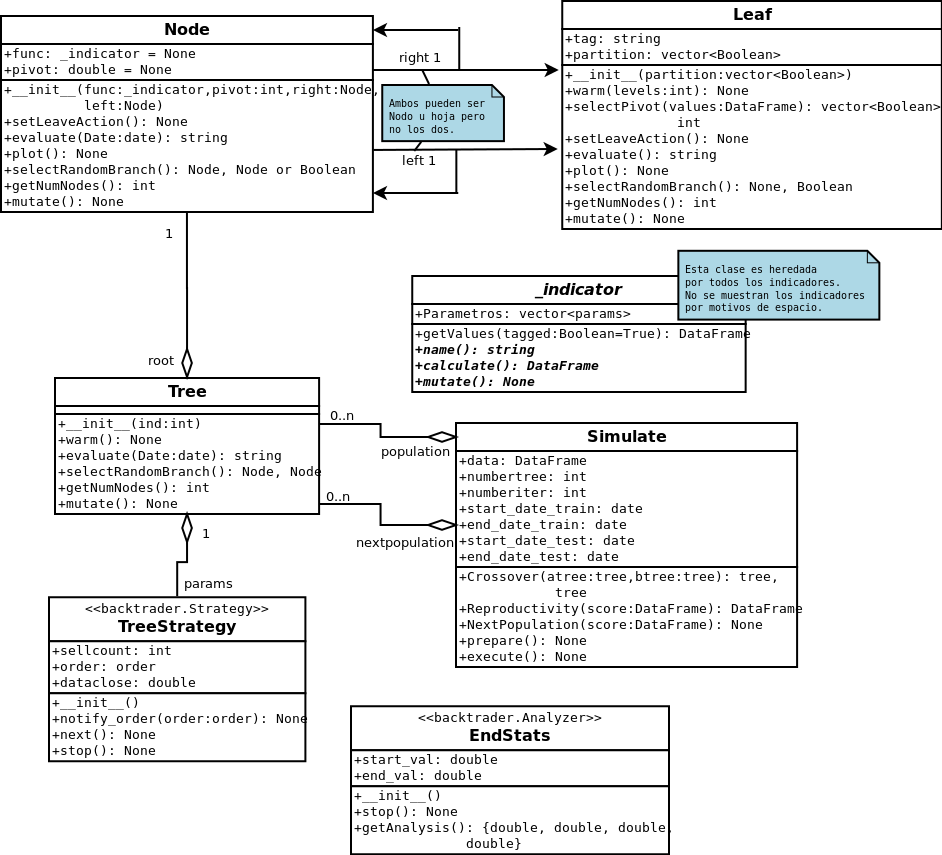
\includegraphics[scale=0.60]{imagenes/diagramaClases.png}
    	    \caption[Diagrama de clases del software desarrollado.]{Diagrama de clases del software desarrollado.\\ Fuente: elaboraci\'on propia}
    		\label{fig:diagclases}
	   \end{figure}

\subsection{Optimizaciones}\label{sec:timeimprove}

Los algoritmos evolutivos suelen tener unos buenos resultados, no solo por su caracter natural, si no por su amplia capacidad para inspeccionar el espacio de b\'usqueda cercano a las buenas soluciones.\\

En espacios de b\'usqueda amplios, como es el caso, las combinaciones son muy grandes y las b\'usquedas se alargan mucho. A esto hay que a\~nadirle el peso de la funci\'on \textit{fitness} que, en este caso, conlleva simular un periodo de bolsa y evaluar muchas veces los indicadores en distintas fechas. Ade\'as, se dispone de una m\'aquina bastante modesta para su ejecuci\'on.\\

Todos estos inconvenientes hacen necesario poner especial cuidado a la hora de realizar el software e intentar reducir el gasto de tanto tiempo como espacio. Si bien este \'ultimo, en principio, no nos producir\'a problema.\\

\subsubsection{Paralelizaci\'on}
Al utilizar \textit{backtrader} en la introducci\'on (v\'ease \ref{sec:backtrader}) se mostraron varios ejemplos sencillos de uso. Pero el paquete dispone de otras opciones que permiten adaptarlo a nuestras necesidades. Se comentar\'a, a continuaci\'on, la posibilidad de ejecutar en paralelo.\\

Lo primero que se debe reformular para poder ejecutar en paralelo es la estrategia. Como se concret\'o, la clase \textit{cerebro} recibe una estrategia como par\'ametro, que es quien d\'a las se\~nales de compra y venta. De esta forma, si se simulase cada uno de los \'arboles de la poblaci\'on, digamos 50, se tendr\'ian que crear 50 cerebros, a\~nadir 50 veces los datos y simular 50 veces las mismas fechas (cada vez con un individuo distinto).\\

Para corregir este comportamiento, se sugiere usar la funci\'on \textit{optstrategy} de la clase \textit{cerebro} de la siguiente forma:\\

\begin{lstlisting}
cerebro.optstrategy(TreeStrategy,tree=list(population))
\end{lstlisting}

En realidad, esta funci\'on est\'a pensada para a\~nadir una rejilla de par\'ametros que matizan la estrategia definida. En lugar de esto, nosotros vamos a pasar la propia poblaci\'on de \'arboles como rejilla de par\'ametros.\\

Una vez realizado este cambio, Backtrader ejecutar\'a la estrategia con los distintos \'arboles de forma iterativa. No es necesario cargar los datos m\'ultiples veces, basta con una sola copia de estos.\\

Ahora vamos a eliminar la linealida de ejecuci\'on. Backtrader permite ejecutar de forma paralela una estrategia a la que se ha aportado una rejilla de par\'ametros. Con la directiva \textit{cerebro = bt.Cerebro(maxcpus=None)} indicamos que no hay l\'imite de n\'ucleos para la ejecuci\'on. \\

La m\'aquina usada dispone de 4 n\'ucleos. Esto nos da una mejora signficativa de tiempo, ya que nos permite evaluar 4 individuos a la vez. Cuantos m\'as n\'ucleos tenga la m\'aquina, m\'as acentuada ser\'a la mejora.\\


\subsubsection{Cach\'e para indicadores de primer orden}
La parte computacional m\'as costosa es la evaluaci\'on de los indicadores. El c\'alculo de algunos de ellos depende de los valores de la acci\'on de varios d\'as atr\'as. Cargar esos datos y hacer las operaciones repetidas veces es un gasto innecesario de tiempo.\\

Adem\'as los \'arboles tienen varios niveles de profundidad. Para cada d\'ia que se simule la inversi\'on se calculan la misma cantidad de indicadores que de niveles.\\

En un intento de reducir esto, se va usar el paquete de python TA-Lib\footnote{\url{https://mrjbq7.github.io/ta-lib/doc_index.html}. \'Ultima consulta 25 de Julio de 2019}.
TA-Lib es un paquete de c\'alculo para indicadores t\'ecnicos de bolsa. Este software est\'a pensado para calcular un gran n\'umero de indicadores de bolsa a lo largo de un periodo, es decir, aportados los valores de un periodo de tiempo, te devuelve el indicador en el mismo periodo.\\

Un caso de uso ser\'ia el siguiente, en el que se calcula el indicador EMA:\\

\begin{lstlisting}
data['EMA'] = talib.EMA(df['Close'], period)
\end{lstlisting}

La fuerza de este paquete reside en la capacidad de calcular indicadores en espacios de tiempo grande. Para sacar partido de este hecho, en lugar de ir calculando los indicadores en los d\'ias que nos interesan, se va a optar por calcularlo en todos los d\'ias del periodo.\\

Se realiza entonces un \textit{DataFrame} en el que se van almacenando todos los indicadore calculados. Cada vez que se quiere acceder a un indicador en una fecha, primero se comprueba si est\'a ya calculado y, en caso negativo, se calcula y se guarda. Este almac\'en puede perdurar incluso entre distintas generaciones, ya que los \'arboles deber\'ian tener indicadores con par\'ametros iguales o similares.\\ 

De forma sistem\'atica, cuando se requiera un indicador, se acceder\'a la funci\'on \textit{getValues} de cada indicador, que mantiene esta estructura de guardado de datos:\\

\begin{lstlisting}
def getValues(self):
	if self.name() in df.columns.values:  # df es global
		return df[self.name()]
	else:
		return self.calculate()
\end{lstlisting}

Para guardar los datos, cada columna se ha nombrado de forma \'unica para cada indicador. El nombre se conforma por el nombre del indicador y los par\'ametros que hubiere.\\

\subsubsection{Cach\'e para indicadores de segundo orden}

La primera cach\'e elimina coste computacional calculando los indicadores en todas las fechas de una sola vez. Ahora surge un problema provocado por este hecho, cada d\'ia hay que acceder a los indicadores de ese d\'ia en unas 4 o 5 ocasiones (una por nivel de profundidad).\\

Por consiguiente, se van a producir en la simulaci\'on del mismo d\'ia varias b\'usquedas en un \textit{DataFrame} cuyo \'indice son fechas. A priori, se podr\'ia pensar que buscar por fechas es igual que buscar por un entero, pero no es as\'i. Python tiene un tipo especial para tratar con fechas que hace que las b\'usquedas se realenticen mucho.\\

Para evitar esta coste adicional de b\'usqueda, se propone realizar un segundo nivel de cach\'e. En esta ocasi\'on, este almac\'en va a guardar los indicadores del \'ultimo d\'ia del que se pidi\'o un indicador. \\

Como en el mismo d\'ia se va a requerir el uso de varios indicadores, estamos ahorrando b\'usquedas en el \textit{DataFrame} que conforma la primera cach\'e.\\

     	\begin{figure}[H]
    		\centering\leftskip=-30px
    		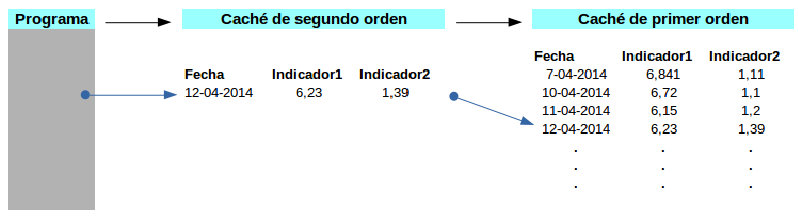
\includegraphics[scale=0.60]{imagenes/caches.png}
    	    \caption[Estructura de las cach\'es]{Estructua de las cach\'es.\\ Fuente: elaboraci\'on propia}
    		\label{fig:caches}
	   \end{figure}
	   
El c\'odigo sigue la misma idea que el desarrollado para la primera cach\'e, solo hay que tener en cuenta que es necesario hacer una nueva variable global para guardar los datos del d\'ia. Adem\'as, ahora la cach\'e puede fallar por dos motivos distintos. El primero que el indicador no est\'e en la primer cach\'e, por tanto es necesario calcular los valores del indicador e incluirlos en el \textit{dataframe}. Y el segundo, que los datos guardados en la segunda cach\'e sean de otro d\'ia, en cuyo caso es necesario cargar el d\'ia correcto en \'esta.\\

\begin{lstlisting}
def getValueByIndex(index, func):
	global thisday
	if func.name() in thisday.columns.values:
		if thisday.index != index:
			thisday = df.loc[[index]]
		return thisday[func.name()][0]
	ret = func.getValues(False).loc[index]
	thisday = df.loc[[index]]
	return thisday[func.name()][0]
\end{lstlisting}

\newpage
\section{An\'alisis de resultados}\label{sec:analisis}
Una vez que el algoritmo est\'a totalmente desarrollado y es funcional, se lanzan un compendio de ejecuciones con distintas combinaciones de par\'ametros con el objetivo de ver cu\'an bueno es.
En un intento de mejorar la comprensi\'on de todas las ejecuciones realizadas, se va a dividir esta secci\'on en dos ep\'igrafes. \\

En el primero de ellos se hace un an\'alisis de los resultados obtenidos haciendo variaciones en los par\'ametros del algoritmo gen\'etico. Estos son el n\'umero de \'arboles, el n\'umero de iteraciones y el tipo de periodo.\\

M\'as tarde, en el segundo ep\'igrafe, se van a comparar los resultados obtenidos, a trav\'es de los mejores par\'ametros, con otro algortimo de naturaleza parecida desarrollado en un art\'iculo.\\


\subsection{An\'alisis de par\'ametros}

Para medir el rendimiento del algoritmo en distintas situaciones, se han propuestos varios periodos de diferente longitud y que presentan distintas tendencias. Por sencillez, todos han sido seleccionados del mismo valor de bolsa, \textit{Banco Santander}.\\

Para obtener una mejor comprensi\'on, se han definido cinco configuraciones de par\'ametros. Cada configuraci\'on tiene sus par\'ametros establecidos en la figura \ref{fig:params}. Estas configuraciones, dependiendo de la longitud del periodo, pueden tardar desde unos minutos en ejecutar hasta cuatro horas en el caso m\'as grande.\\

     	\begin{figure}[H]
     		\centering\leftskip=52px
     		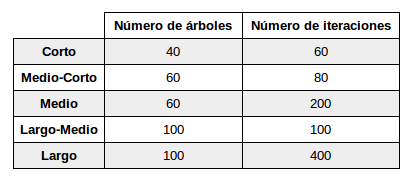
\includegraphics[scale=0.65]{imagenes/params.png}
     		\caption[Configuraciones de par\'ametros]{Configuraciones de par\'ametros.\\ Fuente: elaboraci\'on propia}
     		\label{fig:params}
     	\end{figure}

N\'otese que estas aproximaciones de tiempo ejecuci\'on se aportan a partir de la m\'aquina disponible, en este caso, de cuatro n\'ucleos y 3.4GHz.\\

En los casos expuestos a continuaci\'on se sigue siempre el mismo procedimiento. En primer lugar, el algoritmom gen\'etico efect\'ua, con los par\'ametros correspondientes, una serie de ejecuciones que terminan con una poblaci\'on evolucionada. De esta poblaci\'on obtenida, se selecciona el mejor de los individuos y se prueba tanto en el periodo de entrenamiento como en el periodo de prueba.\\

\subsubsection{Perido largo}

En la primera de las ejecuciones, el periodo de entrenamiento comprende desde el 1 de abril de 2012 hasta el 1 de enero de 2016, por tanto, corresponde con un periodo bastante largo. De forma coherente, el periodo de prueba empieza el 1 de enero de 2016 y finaliza el 1 de mayo de 2019. Al comparar los perfiles de los precios en sendos periodos en las gr\'aficas, que se muestran a continuaci\'on, se puede observar que son parecidos, lo que deber\'ia mejorar los resultados.\\

     	\begin{figure}[H]
     		\centering\leftskip=-75px
     		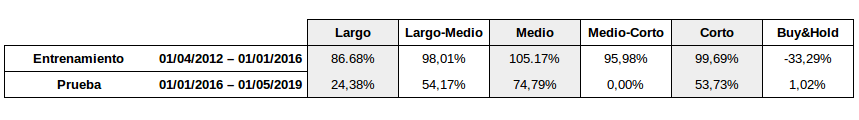
\includegraphics[scale=0.60]{imagenes/Large_period.png}
     		\caption[Ejecuci\'on en un periodo largo ascendente-descendente]{Ejecuci\'on en un periodo largo ascendente-descendente. Las cantidades mostradas son el porcentaje de beneficio respecto al presupuesto inicial.\\ Fuente: elaboraci\'on propia}
     		\label{fig:large_period}
     	\end{figure}
     	
A priori puede parecer que los resultados, que se pueden ver en la figura \ref{fig:large_period} son muy buenos. Pero, en realidad, muestran algunas carencias que se hacen obvias cuando se ve el calendario de inversi\'on.\\

Lo primero que destaca en la figura \ref{fig:large_period_mtrain}, que representa el calendario de inversi\'on del algoritmo con par\'ametros de perfil medio, es que la gran mayor\'ia de las ganancias proviene de una \'unica compraventa. El resto de inversiones son de poca duraci\'on y apenas si producen ganancias. La causa de este hecho puede ser una falta de especializaci\'on. A lo largo de la ejecuci\'on, alg\'un \'arbol ha conseguido hacer esa transacci\'on tan ventajosa y, a partir de esta, no se ha conseguido mejorar pr\'acticamente nada.\\

Es claro que, una inversi\'on de compra y venta algo m\'as r\'apida nos habr\'ia aportado una mayor ganacia.\\

Cuando analizamos el periodo de prueba, representado en la figura \ref{fig:large_period_mtest}, obtenemos un perfil similar. Se ha ajustado de manera muy eficiente una \'unica compraventa. Si bien es cierto que esa transacci\'on es casi perfecta, hay otras transacciones v\'alidas que no se han ejecutado.\\

     	\begin{figure}[H]
     		\centering\leftskip=30px
     		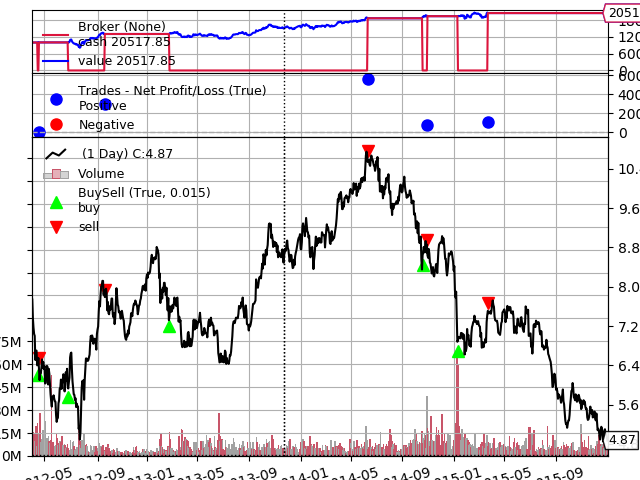
\includegraphics[scale=0.72]{imagenes/L_Medium_train.png}
     		\caption[Calendario de inversi\'on del periodo de entrenamiento largo.]{Calendario de inversi\'on del periodo de entrenamiento largo con par\'ametros de perfil Medio.\\ Fuente: elaboraci\'on propia}
     		\label{fig:large_period_mtrain}
     	\end{figure}
     	
     	\begin{figure}[H]
     		\centering\leftskip=30px
     		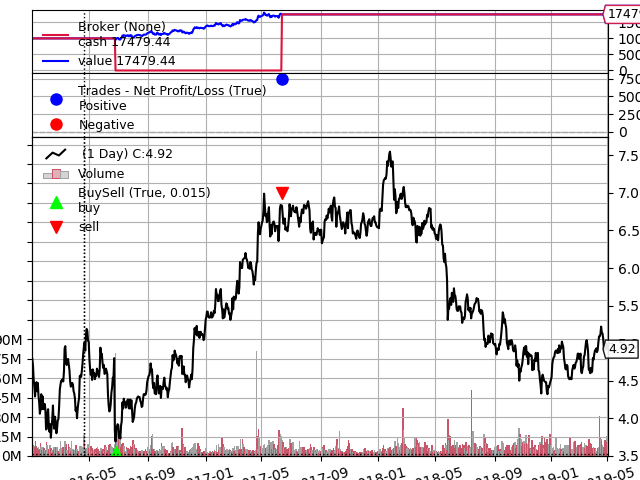
\includegraphics[scale=0.72]{imagenes/L_Medium_test.png}
     		\caption[Calendario de inversi\'on del periodo de prueba largo]{Calendario de inversi\'on del periodo de prueba largo con par\'ametros de perfil Medio.\\ Fuente: elaboraci\'on propia}
     		\label{fig:large_period_mtest}
     	\end{figure}     	

En resumen, los peridos largos dan muchas posibilidades de compraventa que nuestro algoritmo no sabe aprovechar. La parte positiva es que la mayor\'ia de las veces, cuando invierte, lo hace con beneficio. No obstante, en ocasiones, puede que no invierta y tengamos un modelo f\'util, como es el caso de la ejecuci\'on de par\'ametros de perfil Medio-Corto.\\

\subsubsection{Perido medio}

En este segundo caso, se han elegido dos periodos distintos. En el primer periodo, claramente alcista, el entrenamiento comprende desde el 29 de septiembre de 2002 hasta el 29 de septiembre de 2003. Por otro lado, el periodo de prueba empieza el 29 de septiembre de 2003 y finaliza el mismo d\'ia de 2004. \\

El segundo periodo, de car\'acter bajista, esta formulado tambi\'en de a\~no en a\~no, el entrenamiento se comienza el 1 de noviembre de 2009 y la prueba empieza el 1 de noviembre de 2010.\\

Una vez m\'as, se han tomado fechas en las que los perfiles de los precios se asemejan. \\

     	\begin{figure}[H]
     		\centering\leftskip=-75px
     		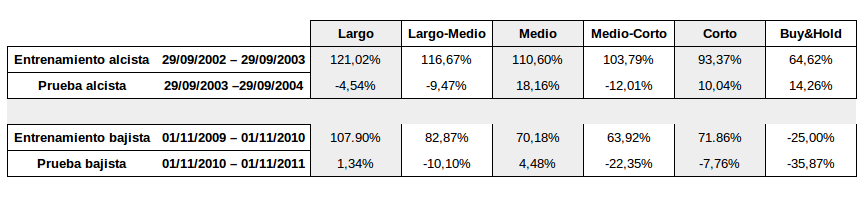
\includegraphics[scale=0.60]{imagenes/Medium_period.png}
     		\caption[Ejecuciones en un periodo medio alcista y en un periodo medio bajista]{Ejecuciones en un periodo medio alcista y en un periodo medio bajista. Las cantidades mostradas son el porcentaje de beneficio respecto al presupuesto inicial.\\ Fuente: elaboraci\'on propia}
     		\label{fig:medium_period}
     	\end{figure}
     	
En esta ocasi\'on, los resultados son significativamente peores. Con motivo de ilustrar la adaptaci\'on de los modelos obtenidos en el periodo de entrenamiento, se han tomado periodos de prueba ligeramente peores, es decir, el precio tiende, significativamente, a bajar m\'as que en el entrenamiento.\\

En todos los casos, el modelo obtenido con el algoritmo gen\'etico fue mejor que la estrategia \textit{Buy\&Hold} evaluados en el periodo de entrenamiento. Esto quiere decir que el algoritmo es capaz de encontrar condiciones de compra y venta que reportan beneficios en el periodo de aprendizaje. Sin embargo, estas condiciones no devuelven buenos resultados en periodos ligeramente distintos. De hecho, incluso en periodos alcistas, se pierde dinero cuando el modelo en el entrenamiento consigue sacar un 121.02\% de beneficios.\\

Otro punto que se puede destacar es la irregularidad del algoritmo. Habitualmente, otros algoritmos tienden a sobreaprender cuando se insiste demasiado en los datos de entrenamiento. As\'i pues, es habitual encontrar un punto de entrenamiento a partir del cual los resultados obtenidos en las pruebas empeoran.\\

En este algoritmo propuesto, los resultados obtenidos  para el periodo de prueba parecen variar de forma independiente al periodo anterior. Tras m\'ultiples ejecuciones con los mismos par\'ametros se puede observar como, en ocasiones, los resultados var\'ian de forma significativa. Este hecho puede ser la causa de una alta aleatoriedad en algoritmo debida a, posiblemente, la gran cantidad de mutaciones necesarias y la aleatoriedad de la primera generaci\'on.\\

     	\begin{figure}[H]
     		\centering\leftskip=40px
     		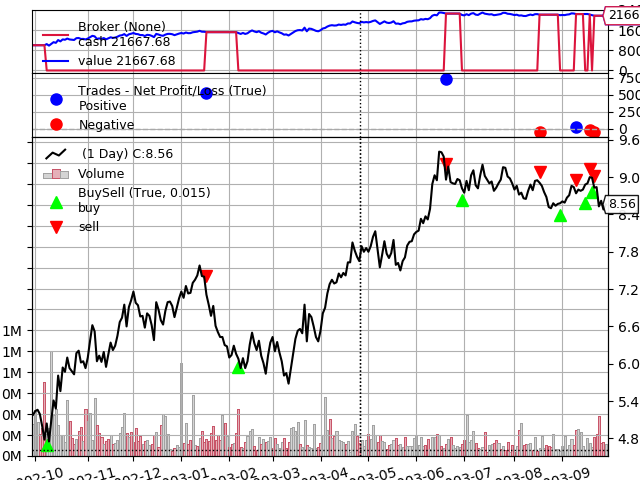
\includegraphics[scale=0.66]{imagenes/M_Large-Medium_train.png}
     		\caption[Calendario de inversi\'on del periodo de entrenamiento largo.]{Calendario de inversi\'on del periodo de entrenamiento medio con par\'ametros de perfil Medio-Corto.\\ Fuente: elaboraci\'on propia}
     		\label{fig:medium_period_mtrain}
     	\end{figure}
     	
     	\begin{figure}[H]
     		\centering\leftskip=40px
     		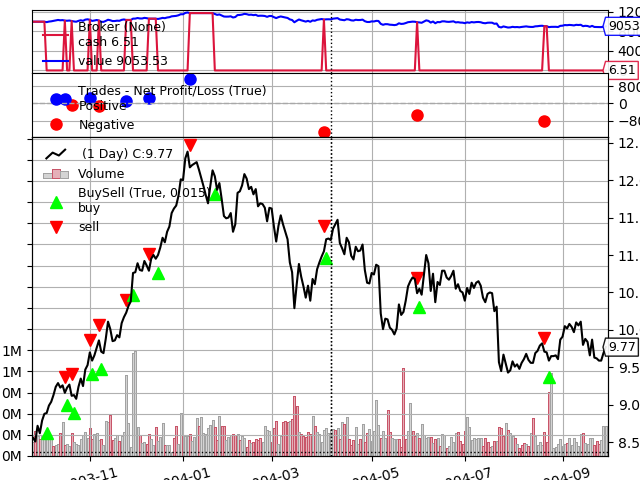
\includegraphics[scale=0.66]{imagenes/M_Large-Medium_test.png}
     		\caption[Calendario de inversi\'on del periodo de prueba medio]{Calendario de inversi\'on del periodo de prueba medio con par\'ametros de perfil Medio-Corto.\\ Fuente: elaboraci\'on propia}
     		\label{fig:medium_period_mtest}
     	\end{figure} 

En las figuras \ref{fig:medium_period_mtrain} y \ref{fig:medium_period_mtest} puede observarse bastante bien esta poca adaptaci\'on. En el periodo de entrenamiento se hacen varias inversiones de unas semanas, e incluso de varios meses, entre las cuales se deja un margen de tiempo hasta que es un buen momento de compra. Por el contrario, en el periodo de prueba apenas si hay unas semanas que el modelo no tiene nada comprado, es decir, siempre que vende intenta comprar inmediatamente.\\

Se considera, en consecuencia a este hecho, la hip\'otesis de que el algoritmo tiene un buen aprendizaje pero una mala adaptaci\'on a otros periodos.\\

     	
\subsubsection{Periodo corto}

Para la \'ultima de las ejecuciones de par\'ametros, se han escogido tambi\'en dos periodos pero, esta vez, se ha tomado un periodo alcista y un periodo lateral. Este segundo es algo complicado, pues el periodo de entrenamiento es lateral pero el de prueba tiene tendencia bajista. \\

En primer lugar, el periodo alcista tiene su entrenamiento desde el 1 de julio de 2016 y hasta el 22 de octubre de 2016. Por otro lado, el periodo de preuba empieza a partir de entonces y hasta el 1 de febrero de 2017.\\

En segundo lugar, el periodo lateral comprende un poco m\'as de tres meses. El periodo de entrenamiento empieza el 1 de enero de 2018 y, por su parte, el periodo de prueba comienza el 22 de abril de 2018. La simulaci\'on termina, finalmente, el 22 de julio de 2018. Como ya se ha adelantado, no se esperan buenos resultados. Los modelos generados tiene poca capacidad de adaptaci\'on y, como hemos tomado periodos de entrenamiento y prueba con perfiles muy distintos, la adaptaci\'on debe ser bastante peor.\\

     	\begin{figure}[H]
     		\centering\leftskip=-75px
     		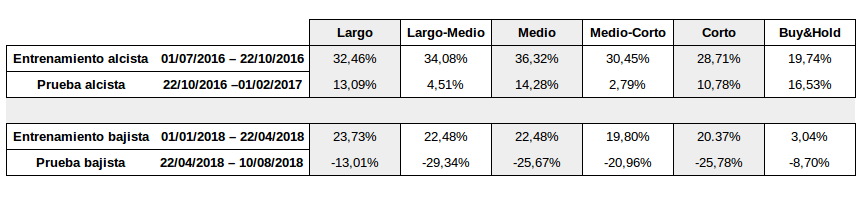
\includegraphics[scale=0.60]{imagenes/Short_period.png}
     		\caption[Ejecuciones en un periodo corto alcista y en un periodo corto lateral]{Ejecuciones en un periodo corto alcista y en un periodo corto lateral. Las cantidades mostradas son el porcentaje de beneficio respecto al presupuesto inicial.\\ Fuente: elaboraci\'on propia}
     		\label{fig:short_period}
     	\end{figure}

Como se observa en la figura \ref{fig:short_period}, en los periodos cortos no se obtienen buenos resultados. De hecho, en el caso del periodo lateral, y prueba bajista, los resultados son p\'esimos. Mientras que, en el entrenamiento, la estrategia propia supera con creces a la estrategia \textit{Buy\&Hold}, en la prueba tiene p\'erdidas estrepitosas al ser un periodo bajista. Esto confirma la hip\'otesis de la baja adaptaci\'on del algoritmo.\\

     	\begin{figure}[H]
     		\centering\leftskip=30px
     		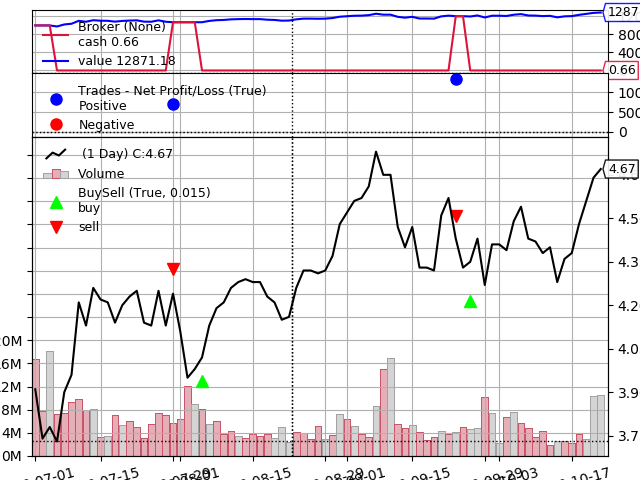
\includegraphics[scale=0.70]{imagenes/S_Short_train.png}
     		\caption[Calendario de inversi\'on del periodo de entrenamiento corto alcista.]{Calendario de inversi\'on del periodo de entrenamiento corto alcista con perfil de par\'ametros Corto.\\ Fuente: elaboraci\'on propia}
     		\label{fig:short_period_uptrain}
     	\end{figure}
     	
En la figura \ref{fig:short_period_uptrain}, correspondiente al periodo alcista de entrenamiento, se encontra un modelo generado con perfil de par\'ametros corto que invierte de una forma muy eficiente, esto es, compra en los m\'inimos y vende en los m\'aximos. \\

Teniendo esta regla como referencia, se analiza el mismo modelo ejecutado, esta vez, en el periodo de prueba en la figura \ref{fig:short_period_uptest}. Este periodo tiene un perfil de precio distinto, los m\'inimos y m\'aximos no son tan destacables. No obstante, el algoritmo ha generado un modelo que, tal y como se intuye, esta intentando hacer algo similar a lo realizado en el periodo del que aprendi\'o. Las primeras transacciones son torpes y demasiado abundantes, produciendo p\'erdidas con las comisiones.	Por tanto, a pesar de ser un periodo alcista, no tiene tanto \'exito como la estrategia de \textit{Buy\&Hold}.\\
     	
     	\begin{figure}[H]
     		\centering\leftskip=30px
     		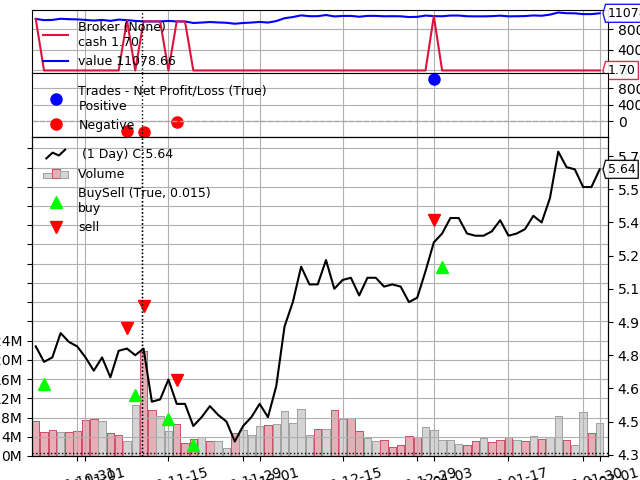
\includegraphics[scale=0.70]{imagenes/S_Short_test.png}
     		\caption[Calendario de inversi\'on del periodo de prueba corto alcista]{Calendario de inversi\'on del periodo de prueba corto alcista con perfil de par\'ametros Corto.\\ Fuente: elaboraci\'on propia.}
     		\label{fig:short_period_uptest}
     	\end{figure} 
     	
Por \'ultimo, se propone hacer una an\'alisis del periodo entrenado con perfil lateral pero probado con un perfil bajista. Las figuras \ref{fig:short_period_uptrain} y \ref{fig:short_period_downtrain} contiene los calendarios de inversi\'on de estas simulaciones realizadas con configuraci\'on de par\'ametros Largo.\\

En el entrenamiento se tiene una inversi\'on muy ajustada, pr\'acticamente inmejorable. No obstante, esto podr\'ia ser fruto de un sobreaprendizaje. Por su parte, en el periodo de prueba, se observan los mismos patrones de compra y venta. Pero al ser las oscilaciones del precio m\'as peque\~nas que en el caso anterior, las comisiones se llevan esos escasos beneficios que pudiera tener.\\

En contraposici\'on, encontramos un punto a favor, la precisi\'on para encontrar los m\'inimos. Los indicadores parecen ser unas buenas herramientas para detectar estos. N\'otese que, tras una acentuada ca\'ida durante el primer mes, se compra en el \'ultimo momento antes de la subida. Por tanto, aunque los resultados no son para nada correctos, las se\~nales de compra y venta no son demasiado err\'oneas. \\
     	
      	\begin{figure}[H]
      		\centering\leftskip=40px
      		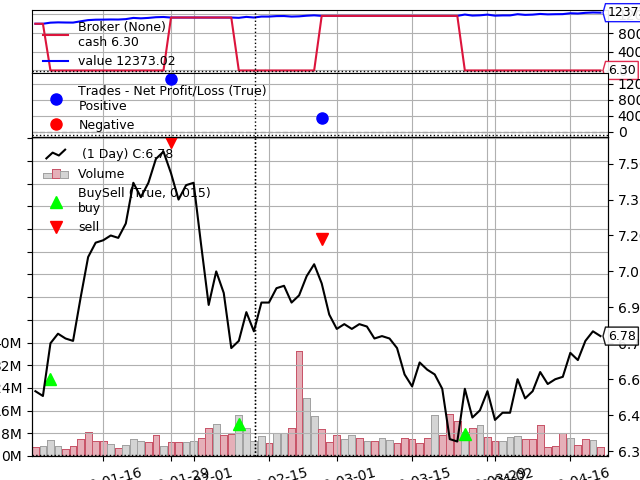
\includegraphics[scale=0.66]{imagenes/S_Large_train.png}
      		\caption[Calendario de inversi\'on del periodo de entrenamiento corto lateral]{Calendario de inversi\'on del periodo de entrenamiento corto lateral con perfil de par\'ametros Largo.\\ Fuente: elaboraci\'on propia.}
      		\label{fig:short_period_downtrain}
      	\end{figure}
      	
     	\begin{figure}[H]
     		\centering\leftskip=40px
     		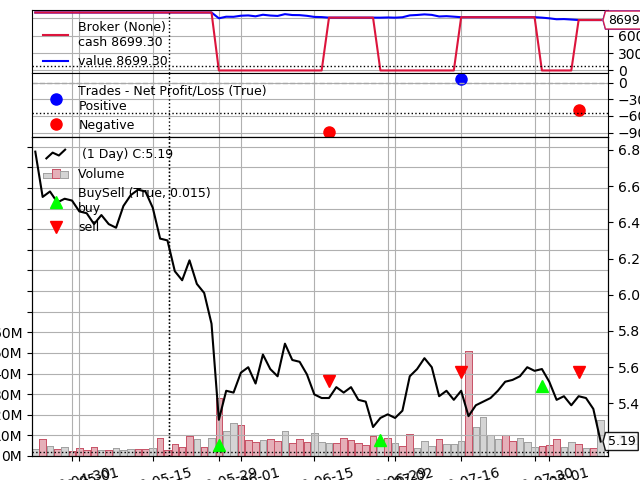
\includegraphics[scale=0.66]{imagenes/S_Large_test.png}
     		\caption[Calendario de inversi\'on del periodo de prueba corto bajista]{Calendario de inversi\'on del periodo de prueba corto bajista con perfil de par\'ametros Largo.\\ Fuente: elaboraci\'on propia.}
     		\label{fig:short_period_downtest}
     	\end{figure} 

\subsection{Contraste con otras estrategias}


\newpage

\section{Conclusiones}
Para finalizar este proyecto, se va a hacer una s\'intesis en la que repasaremos los objetivos que propusimos al inicio.\\

En primer lugar, se prentend\'ia realizar un algoritmo evolutivo basado en \'arboles para extraer informaci\'on de se\~nales de compra y venta. El dise\~no de este algoritmo se especifica en el punto \ref{sec:algorithm}. El c\'odigo que corresponde al dise\~no no se puede incluir en la memoria por motivos de espacio, no obstante, se incluye como anexo.\\

En el segundo punto se propuso implementar mejoras de tiempo para hacer el algoritmo eficiente. Tras las mejoras realizadas en la secci\'on \ref{sec:timeimprove}, el software mostr\'o una reducci\'on de tiempo considerable. En el caso de la ejecuci\'on m\'as larga, entrenamiento de cuatro a\~nos y prueba de tres con poblaci\'on de 100 \'arboles y 400 iteraciones, el tiempo total fue de algo menos de cuatro horas. La ejecuci\'on m\'as corta, por su parte, de tres meses de entrenamiento y otros tres de prueba con 40 \'arboles y 60 iteraciones, tuvo un tiempo de apenas dos minutos. Recordando que las ejecuciones fueron realizadas en un ordenador convencional de cuatro n\'ucleos y 3.4GHz, la eficiencia es satisfactoria.\\

En el tercer punto se marc\'o como objetivo analizar los resultados obtenidos en diferentes situaciones y, asimismo, comparar estos con otros resultados de la bibliograf\'ia. Gracias al desarrollo de la secci\'on \ref{sec:analisis} podemos considerar este objetivo cumplido.\\

Por \'ultimo, se incluy\'o un punto adicional en el que se ped\'ia mejorar los resultados obtenidos en la literatura.\\

(.)\\

(.)\\

(.)\\


\subsection{Perfil del algoritmo}



\subsection{Trabajos futuros}



\newpage

\begin{appendices}
\chapter{Indicadores de bolsa}
En esta secci\'on se entra en profundidad en los indicadores usados en la realizaci\'on de las condiciones situadas en los nodos de los \'arboles de decisi\'on. La intenci\'on de este anexo es, por tanto, dar unas breves explicaciones para caracterizar cada indicador, pero no se entrar\'a en sus distintas interpretaciones cl\'asicas.\\


\noindent\textbf{SMA \textit{(Simple Moving Average)}}\\

Es el indicador m\'as b\'asico y, como su propio nombre indica, es una media aritm\'etica de los \'ultimos valores.\\

Tiene un \'unico par\'ametro que corresponde con el n\'umero de instantes a incluir en la media. As\'i pues, si notamos a $P_i$ como el precio de la acci\'on $i$ instantes atr\'as, el c\'alculo del \textit{SMA} ser\'ia el siguiente:

\[SMA(period) = \frac{\sum\limits_{i=1}^{period}P_i}{period}\]

\vspace{0.5cm}
\noindent\textbf{EMA \textit{(Exponential Moving Average)}}\\

La media m\'ovil exponencial es un indicador parecido al \textit{SMA}. Pero, en esta ocasi\'on, los precios de los instantes anteriores no van a tener el mismo peso en la media, es decir, es una media ponderada. Con este indicador, los valores m\'as cercanos en el tiempo son m\'as importantes.\\

La f\'ormula general del \textit{EMA} viene dada por

\[EMA(period) = K_{period} * P_0 + (1 - K_{period}) * EMA_{[-1]}\]

donde $P_0$ es el valor actual de la acci\'on, $EMA_{[-1]}$ es el valor del $EMA$ en el instante anterior y $K_{period} \in (0,1)$ es un valor que depende del periodo escogido. Habitualmente, se toma $K_{period} = \frac{2}{period + 1}$. 

\vspace{0.5cm}
\noindent\textbf{MACD \textit{(Moving Average Convergence Divergence)}}\\

El nombre de este indicador es algo confuso ya que realmente no es un media, sino una diferencia de medias. En concreto, es la diferencia de dos \textit{EMA} de periodo distinto.\\

En consecuencia, \textit{MACD} tiene dos par\'ametros, los periodos de las dos medias exponenciales. El periodo peque\~no debe ser extrictamente menor que el periodo grande.

\[MACD(period_h, period_l) = EMA(period_l) - EMA(period_h)\] 

\vspace{0.5cm}
\noindent\textbf{ATR \textit{(Average True Range)}}\\

Este indicador intenta medir la volatilidad\footnote{La volatilidad es un concepto burs\'atil que hace referencia a la rapidez con la que cambia un determinado valor en un periodo fijo de tiempo. Una volatilidad alta suele ser s\'intoma de inseguridad en los inversores o de un cambio de tendencia.} del precio de la acci\'on. Para ello toma un par\'ametro, el periodo, que ser\'a el que marcar\'a la longitud del intervalo. Es necesario tener, para cada instante del periodo, el precio m\'as alto ($H$), el precio m\'as bajo ($L$) y el precio de cierre ($C$). Se define, entonces, el \textit{TR (True Range)} como 

\[TR = max\{ H-L, |H-C|, |L-C|\}\]

Una vez calculado este valor para todos los instantes del periodo, el \textit{ATR} viene dado por

\[ATR(period) = \frac{1}{period}\sum\limits_{i=0}^{period-1}TR_{i}\]

donde $TR_{i}$ es el \textit{True Range} $i$ instantes atr\'as.

\vspace{0.5cm}
\noindent\textbf{ROC \textit{(Price Rate Of Change)}}\\

El indicador \textit{ROC} nos da un porcentaje de cambio del precio de la acci\'on respecto de un instantes anterior. Tiene un solo par\'ametro, llamado periodo, que indica la distancia del instante anterior a tomar respecto del instante actual.\\

Para calcular este indicador podemos usar la f\'ormula siguiente, donde $C$ es el valor de cierre del instante actual y $C_{period}$ es el valor de cierre del instante $period$ veces atr\'as.

\[ROC(period) = \frac{C - C_{period}}{C_{period}}\]

\end{appendices}

\newpage
\printbibliography[title=Bibliografía, heading=bibintoc]


\end{document}
